\chapter[Modelado de la Geometría de Miga de Pan]{Modelado Procedimental de Geometrías de Miga de Pan y Otros Materiales Porosos}

\section{Introducción y Motivación} % (Películas de Animación)
Como fue previamente explicado, determinados materiales recibieron menor atención en la literatura científica, debido entre otros factores, a la dificultad en el modelado, a los altos costos computacionales, y/o a la necesidad de utilización del material en aplicaciones prácticas.
Con el paso de los a\~nos, la industria del cine y de los video juegos utilizó procedimientos artísticos que intentan subsanar estas deficiencias.
De esta forma, se busc\'o la mayor similitud posible entre el material sintetizado y el real, sin importar si el proceso es una simulación física o el resultado de un procedimiento artístico.
Entre los innumerables ejemplos que se pueden citar, uno particularmente relacionado al trabajo de esta tesis lo constituye la película Ratatouille \cite{Cho2007}.
La misma se desarrolla en un ambiente de cocina, y por lo tanto existen alimentos y materiales naturales que deben ser modelados para ser renderizados.
Debido a la inexistencia de modelos estándar de determinados materiales en la literatura de computación gráfica (comestibles), los artistas y programadores encargados de llevar a cabo la producción visual de la película debieron crear técnicas ad-hoc para lograr un renderizado realista de los diferentes materiales.
Sin embargo, el éxito visual obtenido no se vio acompañado de una liberación del código que producía dichas imágenes, por lo cual la técnica permaneció para uso privado de la compañía productora, resultando en una difícil reproducción de dichos materiales por parte de terceros.

En nuestro trabajo intentamos subsanar estas deficiencias.
Por un lado, la falta de modelos ad-hoc documentados y por lo tanto reproducibles, y por otro, la utilización de modelos físicos basados en los procesos reales de formación de los materiales, los cuales sin dudas provocarán que el resultado sintético posea una mayor similitud visual y estructural a los materiales que se pretenden representar.

\section{Un Framework para la Síntesis de Texturas de Materiales}
En primer lugar presentaremos un sencillo procedimiento, en dos dimensiones, que permite obtener texturas de distintos materiales.
Dichos materiales usualmente se presentan en publicaciones separadas en la literatura, dado que los procedimientos que producen las mismas son fuertemente diferentes.
El procedimiento presentado ser\'a luego derivado para obtener texturas de pan y otros materiales porosos.

%Una vez establecidas las texturas en computación gráfica como un método simple y eficiente de representar materiales, se idearon técnicas automáticas para generarlas.
%De esta forma, no se depende exclusivamente de imágenes para obtener las mismas.

\subsection{Sistemas de Partículas y Autómatas Celulares}
En un sistema de part\'iculas \cite{Reeves1983} t\'ipico las part\'iculas nacen, se desarrollan y mueren, respetando reglas que les son impuestas por el sistema. Estos sistemas intentan modelar la din\'amica del fen\'omeno a trav\'es del tiempo, siendo uno de sus principales intereses mostrar una animaci\'on del mismo \cite{Gao2010, Bagar2010, Lentine2010}.

Se propone utilizar estos sistemas como generadores procedimentales de texturas. Un enfoque similar puede observarse en \cite{Kranidotis98}, aunque el mismo no fue desarrollado en profundidad.
Aquí se sigue una linea de investigaci\'on similar, presentando un sistema de part\'iculas que est\'a caracterizado por el crecimiento de las mismas en cada iteraci\'on, las cuales ocupan texels asign\'andoles colores, pudi\'endose detener al mismo en la iteraci\'on que se crea conveniente, obteni\'endose una textura.
Las im\'agenes resultantes presentan aleatoriedad, lo cual es deseable en materiales naturales.
A trav\'es de la direcci\'on de crecimiento de las part\'iculas se producen distintos patrones visuales.

Es posible representar materiales cl\'asicos como madera, granito y m\'armol, pero tambi\'en otros como mosaicos, pinturas, vegetaci\'on, entre muchos otros.
En un trabajo anterior \cite{Baravalle2010} se abord\'o la generaci\'on procedimental de texturas.
La diferencia radica en el mecanismo de generaci\'on, dado que con esta nueva propuesta es un {\em proceso temporal} el que produce los resultados, con lo cual puede representarse todo el proceso de formaci\'on de un material.
Adem\'as, cada corrida del algoritmo produce una textura distinta utilizando los mismos par\'ametros, debido a la naturaleza aleatoria de la generaci\'on (aunque el uso de seeding permitir\'ia repetir texturas en el caso de requerirse, por ejemplo para generar baldosas id\'enticas).

Se utiliza como plataforma de implementaci\'on a WebGL\footnote{\em http://www.khronos.org/webgl/}, recientemente propuesta por el Khronos Group (Open Standars for Media Authoring and Acceleration), dado que la misma otorga portabilidad al modelo. 
Programadores pueden incluirlo como biblioteca en aplicaciones gr\'aficas.
Dise\~nadores pueden utilizar la implementaci\'on para producir materiales, dada la intuitividad de los par\'ametros del mismo.

\subsubsection{Desarrollo}
Inicialmente el sistema consta de un conjunto de part\'iculas $P$
\begin{equation}
P = \{p_{1}, ... , p_{n}\}, n  \in \mathbb{N},
\end{equation}
uno o varios colores {\em RGB}, los cuales pueden tomar las part\'iculas.
\begin{equation}
cols = \{col_{1}, ... , col_{m} \}, m \in \mathbb{N},
\end{equation}
un conjunto de direcciones de crecimiento $D$,
\begin{equation}
D = \{d_{1}, ... , d_{k} \}, k \in \mathbb{N},
\end{equation}
y una grilla $B_{N\times N}, N \in \mathbb{N} $ de texels con colores RGB asociados (inicialmente $(R,G,B)=(0,0,0)$).

Cada elemento del conjunto $P$ posee las siguientes propiedades:
\begin{equation}
p_{i} = \{T_{i}, C_{i}, d_{i}, color_{i}\}, 1 \le i \le n,
\end{equation}
donde:

$T_{i} = \{t_{1}, ... , t_{n_{i}}\}$: conjunto de texels {\em ocupados} por la part\'icula en $B$,

$C_{i} = \{c_{1}, ... , c_{m_{i}}\}$: conjunto de texels {\em contorno} de la part\'icula en $B$,

$d_{i} \in D$: direcci\'on de crecimiento,

$color_{i}$: color {\em RGB} de la part\'icula, con ecuaci\'on \cite{Reeves1983}
\begin{equation}
color_{i} = col_{h} + rand * varcolor,
\label{eqColor}
\end{equation}

\noindent
y donde rand es un n\'umero pseudo-aleatorio uniformemente distribuido entre $-1$ y $1$, $varcolor$ un par\'ametro y $col_{h} \in cols$.
Cada $t \in T_{i}$ tiene asociado un color que var\'ia con respecto a $color_{i}$, de similar manera a la ecuaci\'on (\ref{eqColor}).

El {\em contorno} de una part\'icula determina los texels que la misma puede incorporar. 
En cada iteraci\'on, se elige aleatoriamente un texel en $C_{i}$, se lo quita del mismo y se lo incorpora a $T_{i}$.
Luego se actualiza el contorno de acuerdo a $d_{i}$ y al nuevo texel incorporado.
Se repite el proceso $\forall p_{i} \in P$, respetando las siguientes restricciones:
\begin{eqnarray}
\forall p_{i}, p_{j} \in P, t \in T_{i} \Rightarrow t \notin T_{j}, \\
\forall p_{i} \in P, t \in T_{i} \Rightarrow t \notin C_{i}.
\end{eqnarray}

Es decir, si una part\'icula posee un texel en $T_{i}$, ninguna otra lo posee (las part\'iculas son disjuntas), y si una part\'icula posee un texel en $T_{i}$, \'este no est\'a en su contorno.

Las part\'iculas pueden {\em nacer} y {\em morir}, lo cual representa su inclusi\'on o eliminaci\'on de $P$.
Al morir, la part\'icula deja asociados los colores de su conjunto $T_{i}$ en $B$, pudiendo utilizarse posteriormente esta informaci\'on.

Podemos intentar aplicar estas técnicas al modelado procedimental de texturas. 

En la Fig.~\ref{resultados} se observan algunas im\'agenes sintetizadas.
En la primera fila, la primera y cuarta textura muestran patrones con direcci\'on vertical, direcci\'on elegida para hacer crecer a las part\'iculas.
La \'ultima figura de la segunda fila, muestra part\'iculas que crecen en 3 direcciones posibles: aleatorio ($50\%$), vertical ($25\%$) y horizontal ($25\%$), lo cual demuestra que se posee un control preciso sobre las formas resultantes en las texturas.
En la Figura \ref{sintesis} se observa un ejemplo de s\'intesis.
De izquierda a derecha, se observan texturas obtenidas en las iteraciones $10$, $150$, $250$, $500$ y $1000$.
En la Figura \ref{teteras} se observan texturas sintetizadas aplicadas a un objeto mediante texture mapping, mostrando una calidad aceptable para ser utilizadas en aplicaciones gr\'aficas.
La Figura \ref{muerte} muestra el efecto de muerte de part\'iculas.
Las mismas liberan el espacio en $T_{i}$ dejando asociado su color en $B$, permitiendo que las dem\'as puedan crecer en dichos texels.
De esta forma, puede utilizarse posteriormente la informaci\'on que la misma dej\'o asociada.
En este caso los colores de la part\'icula que libera el espacio y la ocupante fueron mezclados, obteni\'endose im\'agenes que parecen haber sido ``pintadas'' por capas.
%En la Figura \ref{software} se observa el modelo corriendo en un navegador web.


\begin{figure}[t!]
\centering
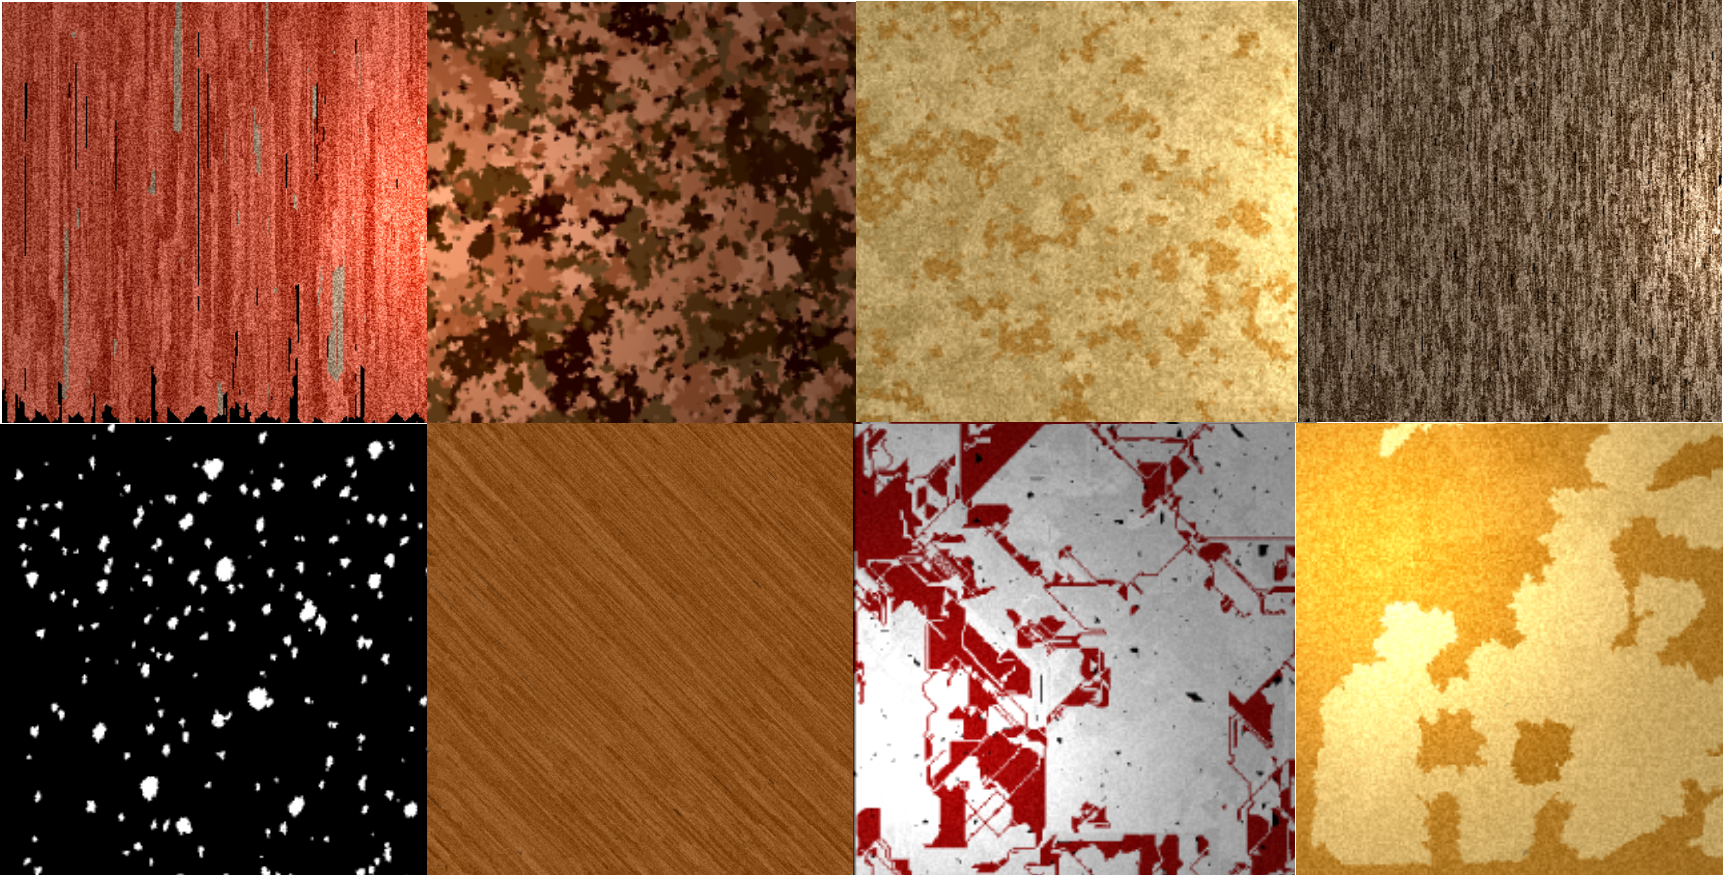
\includegraphics[scale=0.18]{resultados}
\caption{Distintas texturas obtenidas}
\label{resultados}
\end{figure}

Se muestra un ejemplo de s\'intesis de una textura en la Figura \ref{sintesis}. Deben seleccionarse los siguientes par\'ametros:

\begin{itemize}
\item Par\'ametro {\em cantidad de part\'iculas iniciales}, con valor $100$.
\item Par\'ametro {\em nuevas particulas por iteraci\'on}, con valor $1$.
\item Par\'ametros {\em color 1 y 2 (RGB)}. con colores de ejemplo, uno con la componente verde mayor y otro con mayor componente azul.
\item Par\'ametros {\em direcciones}: aleatorio: $50\%$, diagonal $50\%$.
\item Par\'ametro {\em variaci\'on de color}, con valor 0.1, en una escala [0,1] (ver $varcolor$ en la secci\'on anterior).
\item Par\'ametro {\em variaci\'on de color por part\'icula}, con valor 0.1, en una escala $[0,1]$, el cual determina la variaci\'on del color por texel dentro de la part\'icula.
\end{itemize}

\begin{figure}[t!]
\centering
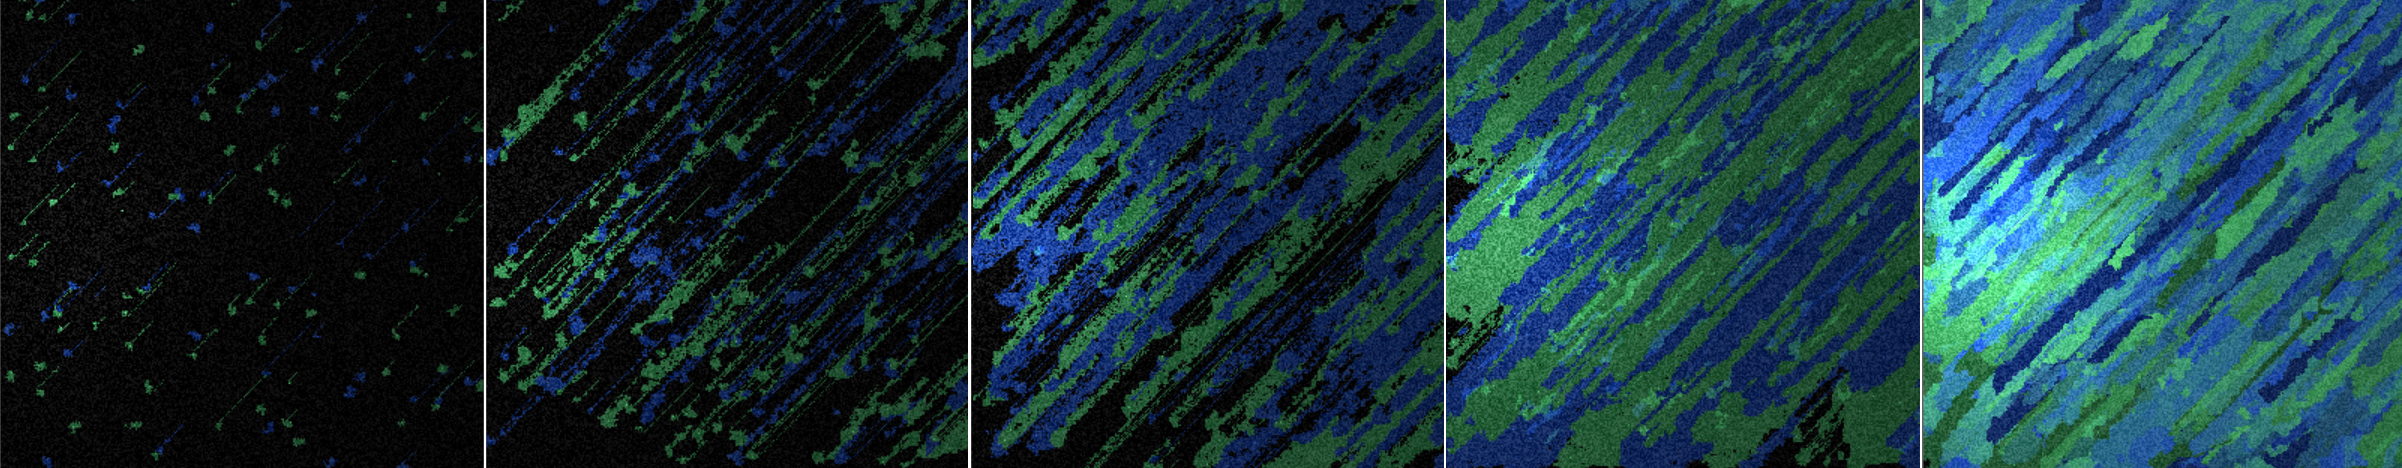
\includegraphics[scale=0.12]{sintesis}
\caption{Ejemplo de s\'intesis de una textura}
\label{sintesis}
\end{figure}

\begin{figure}[t!]
\centering
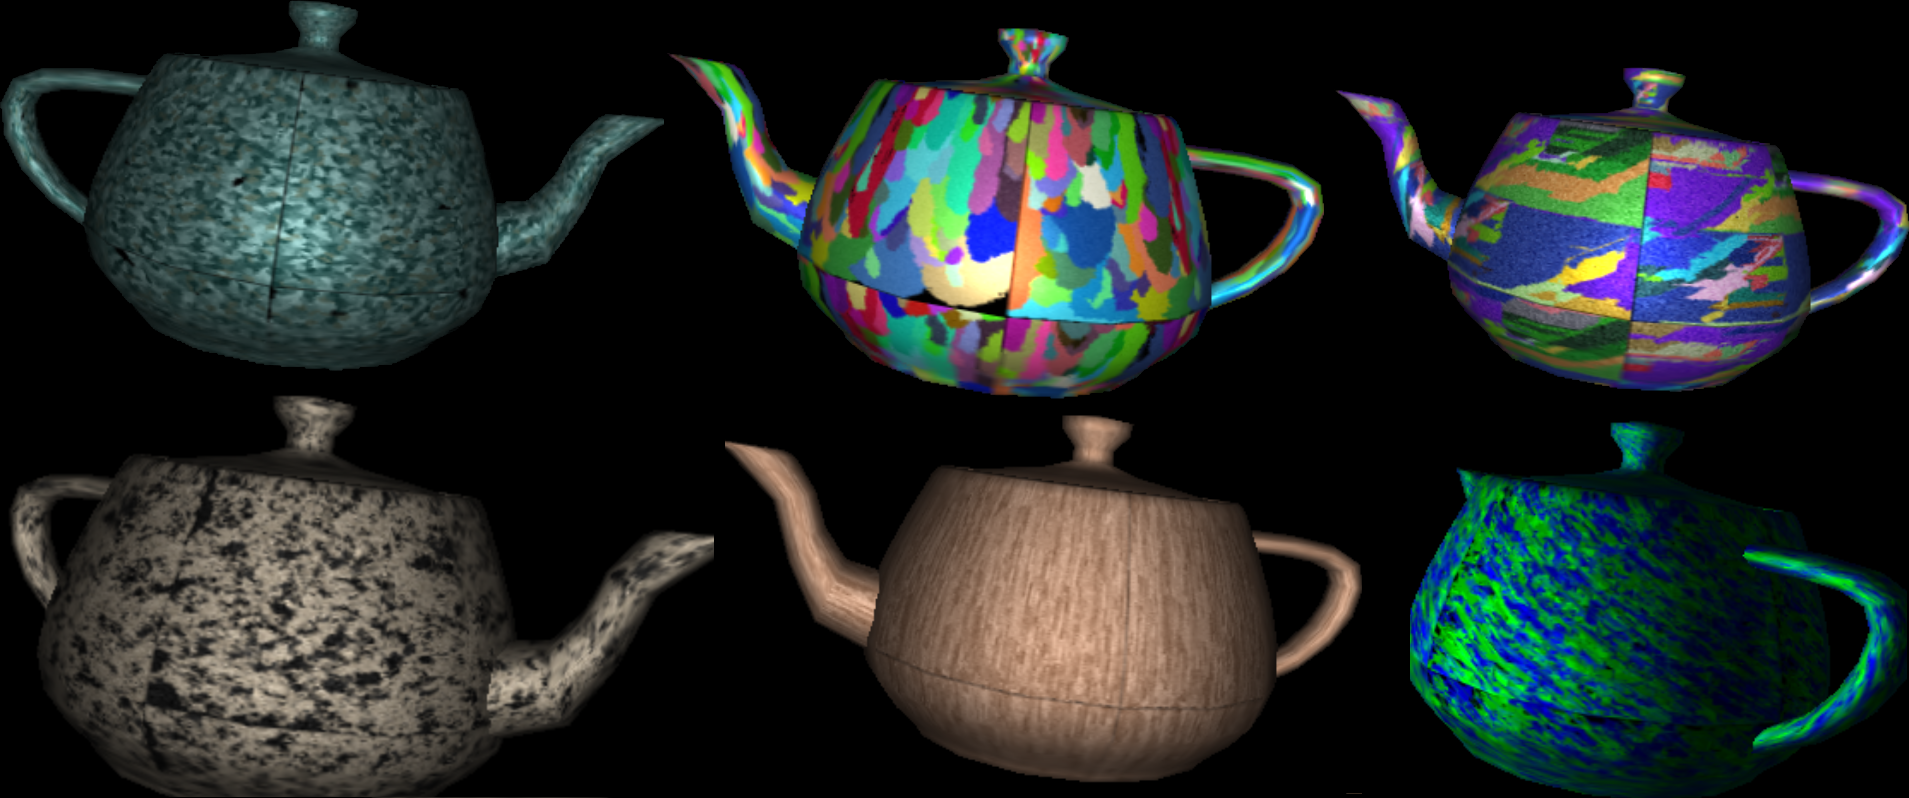
\includegraphics[scale=0.14]{teteras}
\caption{Texturas generadas mapeadas en una tetera}
\label{teteras}
\end{figure}


\begin{figure}[t!]
\centering
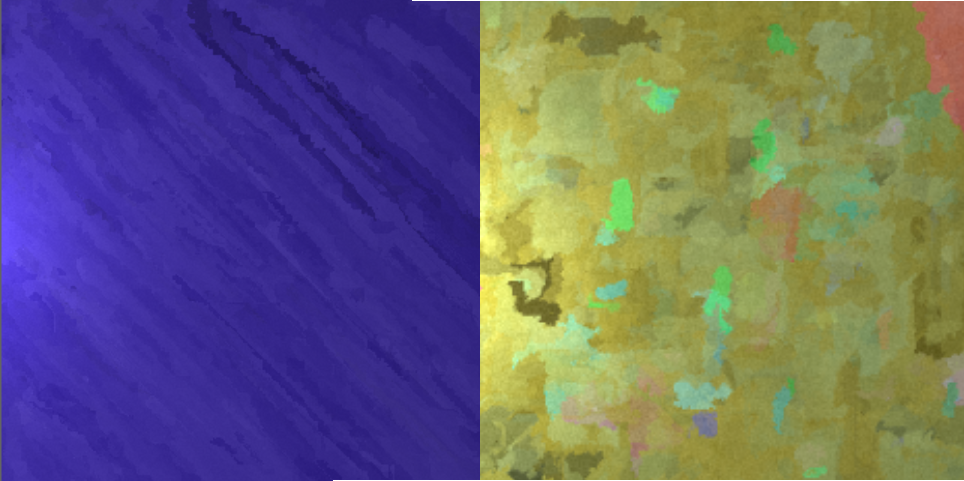
\includegraphics[scale=0.2]{muerte}
\caption{Efecto producido utilizando el concepto de muerte de las part\'iculas}
\label{muerte}
\end{figure}

Los resultados obtenidos muestran una flexibilidad útil para producir distintos materiales.
La idea de utilizar sistemas de partículas para producir materiales será utilizada en la sección siguiente.
Más específicamente para producir geometrías de materiales porosos, particularmente la miga de pan.
Para esto, se generalizarán los resultados a tres dimensiones.

\section{Modelado Procedimental de la Geometría de la Miga de Pan}
En esta sección introducimos un modelo procedimental que permite realizar simulaciones de la geometr\'ia de la miga de pan, basado en el framework introducido en la secci\'on anterior.
Si bien el modelo introducido no está basado en primeros principios, el mismo es un paso previo que permite sentar las bases de un modelo inspirado físicamente.

\subsection{Introducción}
La inmensa variedad de materiales, y sus complejas interacciones con fuentes lumínicas, han sido un tópico central de investigación en las últimas décadas en Computación Gráfica.
El modelado de la naturaleza en física ha demostrado capturar de manera muy precisa fenómenos de transporte de la luz.
Las aproximaciones computacionales a estos modelos son una de las ramas más investigadas en el renderizado de materiales.
El modelado geométrico de materiales sigue una estrategia de investigación similar. Primero se construye un modelo físico del material, el cual luego es aproximado computacionalmente.
Debido a estas observaciones, el renderizado foto-realístico de materiales debe considerar tanto el modelado geométrico de los mismos como su interacción con la luz, para lograr una aproximación adecuada del material.

La elección del modelo geométrico depende de cada material, y de la escala de representación buscada.
Esta elección influencia fuertemente el algoritmo de renderizado. 
Existen dos tipos principales de modelado de materiales: superficies y volúmenes.
Para esto existen dos ecuaciones principales.
Por un lado, la ecuación del rendering \cite{Kajiya1986} captura la microgeometría de los materiales y su interacción con la luz en superficies.
Por otro, la ecuación del rendering de volúmenes \cite{Kajiya1984} modela fenómenos volúmetricos como la transmitancia, la extinción, etc., debido a propiedades del medio (o material).

Si el material a representar es homogéneo (metales, plásticos, y similares), la elección típica es utilizar una superficie para representar el mismo \cite{Neumann1999}.
Esta elección modela la superficie del material asumiendo distribuciones estadísticas en su microgeometría.
Para lograr capturar detalles mesoscópicos, por ejemplo en el caso de maderas o ladrillos \cite{Lefebvre2000}, una técnica usual es precomputar dichas características en texturas, las cuales luego son mapeadas en la superficie.
La utilización de superficies es usualmente menos costosa computacionalmente, pero por otro lado impone limitaciones al realismo que se puede alcanzar, sobre todo en aquellos detalles que son propios de la estructura a nivel mesoscópico y la interacción de la misma con la luz (por ejemplo luz que pasa a través de agujeros en una superficie).

Siguiendo este razonamiento, la miga del pan es un material extremadamente complejo de capturar, modelar y renderizar, debido a la geometría a distintos niveles (microscópico y mesoscópico) y su resultante interacción y fenómenos lumínicos.
De esta forma, la utilización de superficies no es adecuada bajo ningún punto de vista, ya que la textura del pan está dada en gran medida por los fenómenos previamente explicados.
Si bien es cierto que existen métodos en la literatura que utilizan superficies para representar características mesoscópicas de los materiales como funciones de texturas bidireccionales (bidirectional texture functions, BTF) \cite{Tong2002}, las mismas no manejan adecuadamente la interacción lumínica antes mencionada.
Existe un intento en la literatura por suprimir esta falta \cite{Tong2005}.
El método produce imágenes realistas, pero existen muchas dificultades prácticas en la captura, el cómputo y el renderizado.
Estas limitaciones provocan que la utilización de dicho método no sea práctica por el momento.
Además, el método resulta inflexible dado que para cada imagen del material es necesario repetir todo el proceso (dos imágenes distintas del material requieren dos capturas).
Tampoco es posible obtener cortes del mismo, dada la naturaleza de superficie del método.

Por otro lado, existen numerosas publicaciones que tratan el modelado de materiales mejor adaptados a una representación volumétrica (por ejemplo humo o nubes) \cite{Chentanez2011,Zhou2008}.
La utilización de volúmenes es costosa computacionalmente pero presenta varias ventajas. Una de ellas es que no depende de una malla de triángulos, como en el caso de las superficies, y por lo tanto no presenta las desventajas mencionadas para las mismas.

Finalmente, existe un compromiso al momento de modelar materiales complejos y elegir una representación adecuada.
Donde se requiere simplicidad y velocidad (posiblemente tiempo real), se utilizan superficies, en cambio, si el foto-realismo es el objetivo final, es más adecuado optar por una representación volumétrica.
En los últimos años esta elección se ve perturbada por la aparición de hardware paralelo de alta velocidad (placas gráficas o GPUs), ya que un diseño adecuado podría alcanzar imágenes foto-realistas utilizando volúmenes en tiempos interactivos.
Esto es lo que presentaremos a continuación.


En este capítulo proponemos una representación volumétrica para la geometría de la miga de pan, alcanzando incluso tasas de refresco de tiempo real.
Existe un intento similar en la literatura \cite{Perlin1989}, el cual utiliza funciones algebraicas que representan la geometría del material.
En nuestro caso, para ganar flexibilidad de diseño, utilizamos los sistemas de partículas previamente mencionados, en un cubo (tres dimensiones), en conjunto con sistemas dinámicos \cite{Strogatz2001} que provocan una evolución del sistema, produciendo patrones con formas geométricas naturales.
Este es un intento por simular el efecto de la levadura en la masa cruda del pan.
Estos procedimientos producen distribuciones de burbujas de distintos tamaños, resultando en un mecanismo controlable, que presenta propiedades estadísticas.
El sistema es capaz de generar imágenes foto-realistas de diversos tipos de pan, como se mostrará más adelante.

\section{Sistemas Dinámicos como Modelo de Miga de Pan}
El prop\'osito de este algoritmo es producir una geometr\'ia la cual se renderizar\'a posteriormente. Por lo tanto, en lugar de devolver el color de una posici\'on espec\'ifica, el algoritmo genera un campo escalar compuesto de $0$s y $1$s ($0$ si la posici\'on contiene aire, $1$ si la misma contiene masa).
Esta representaci\'on resulta adecuada para ser renderizada utilizando DVR.

El sistema consta de un conjunto de part\'iculas $P$,

\begin{equation}
  P = \{p_{1}, ... , p_{n}\}, n  \in \mathbb{N},
\end{equation}

\noindent una grilla $L_{N\times N \times N}, N \in \mathbb{N} $ (inicialmente $L_{xyz}=1$) de masa y aire como fue descripto previamente, y otra grilla $L^{2}_{N\times N \times N}$, (inicialmente $L^{2}_{xyz}=-1$) de posiciones donde cada celda almacena un único entero que indica qu\'e part\'icula es due\~na de la misma ($i$ si el elemento de la grilla pertenece al contorno o interior de la part\'icula $i$).

Cada elemento en $P$ posee las siguientes propiedades:

\begin{equation}
  p_{i} = \{O_{i}, C_{i}\}, 1 \le i \le n,
\end{equation}

\noindent donde:

\begin{itemize}
\item $O_{i} = \{o_{1}, ... , o_{n_{i}}\}$: (Ocupadas) vector (conjunto) de posiciones ocupadas por la part\'icula en $L$.

\item $C_{i} = \{c_{1}, ... , c_{m_{i}}\}$: (Contorno) vector (conjunto) de posiciones representando el {\em contorno} de la part\'icula en $L$.
\end{itemize}

El vector $O$ representa las posiciones que ser\'an afectadas por la part\'icula, y el contorno $C$ se utiliza para asegurar que las part\'iculas se eviten entre s\'i.

El algoritmo se describe, simplificadamente, en Algoritmo $1$. 

\begin{algorithm}[h!]
\caption{Algoritmo de modelado}
\begin{algorithmic}

\State{$t  = 0$}
\Comment{tiempo - iteración}
\State{$P  = []$}
\Comment{partículas}
\State{$L  = matriz(MxMxM).valores\_iniciales(1)$}
\Comment {Geometría - iniciada a 1 (masa)}
\State{$L^{2} = matriz(MxMxM).valores\_iniciales(-1)$}
\Comment{Dominio de cada partícula}

\For{$i \in [1,Cantidad\_Particulas]$}
    \Comment{Cada partícula toma una posición aleatoria en L}
    \State{$x \gets aleatorio, y \gets aleatorio()$}
    \State{$O[i] \gets [[x,y]]$}
    \State{$C[i] \gets []$}
    \For{$v \in vecindario(x,y)$}
        \State{$C[i].agregar(v)$}
    \EndFor
    \State{$P.agregar([O[i],C[i]])$}
\EndFor

\For {$t \in [0,tiempo\_max]$}
    \For {$i \in [1,Cantidad\_Particulas]$}
        \If {$vacio?~C[i]$}
            \State{morir()}
        \EndIf
        \For{$h \in C[i]$}
            \State{$C[i].eliminar(h)$}
            \Comment{la posición ya fue explorada}
            \State{// Si la posición o el contorno pertenece a otra partícula, elegir otra posición}
            \State{// borde\_libre chequea que el vecindario no este dominado por otra partícula}
            \If{$!(L^{2}[h] > 0 ~\&\&~ L^{2}[h] != i ~\&\&~ borde\_libre(separacion)$}
                \State{// Posición libre, ocupar}                
                \State{$L[h] \gets 0$} \Comment{masa -> aire}
                \State{$O[i].agregar(h)$}
                \State{$C[i].agregar(vecindario(h))$} 
                \State{$L^{2}.setear(vecindario(h),i)$} \Comment{Marcar posiciones en $L^{2}$ como $i$}
                \State{$L^{2}.setear(h,i)$}
                \Comment{turno de la particula $i+1$...}
            \EndIf
        \EndFor
    \EndFor
\EndFor
\end{algorithmic}
\end{algorithm}

Cuando $t = 0$, un conjunto de part\'iculas iniciales toman posiciones aleatorias en la grilla. Para cada partícula, la posici\'on elegida es la primera posici\'on ocupada en $O$, adem\'as, el vecindario de $O$ es agregado a $C$. Cada part\'icula evoluciona en un intento por extender sus posiciones ocupadas ($O$), marcando posiciones en $L$. Las posiciones se toman de $C$. Cuando una part\'icula ocupa una posici\'on, la misma se elimina de $C$ y se agrega a $O$. Luego el vecindario de esa posici\'on se agrega a $C$ (es decir las posiciones que rodean inmediatamente a la posici\'on tomada). Las grillas se actualizan de la siguiente manera: $L$ se setea a $0$ en la posici\'on y $L^{2}$ se setea con el valor $i$ en las posiciones que se agregan a $C$. Las part\'iculas s\'olo pueden crecer si el valor encontrado en $L^{2}$ no pertenece a otra part\'icula. El tama\~no del vecindario es un par\'ametro que define la distancia entre part\'iculas. Si el vector $C$ est\'a vac\'io, la part\'icula {\em muere} ya que no puede continuar creciendo.


El algoritmo puede ser terminado en cualquier $t$ deseado. El mismo puede finalizar su c\'omputo ante determinados eventos, por ejemplo, cuando todas las posiciones de $L^{2}$ fueron tomadas por part\'iculas, ya que no pueden realizarse progresos.

Variando el par\'ametro de distancia entre part\'iculas (separación) se obtienen distintas estructuras (ver Fig.~\ref{fg:sistdin1}). Las im\'agenes muestran ejemplos 2D (para mayor claridad) de crecimiento aleatorio de part\'iculas. La regi\'on blanca en las im\'agenes representa la masa restante luego del proceso.


\begin{figure*}[htb!]
  \centerline{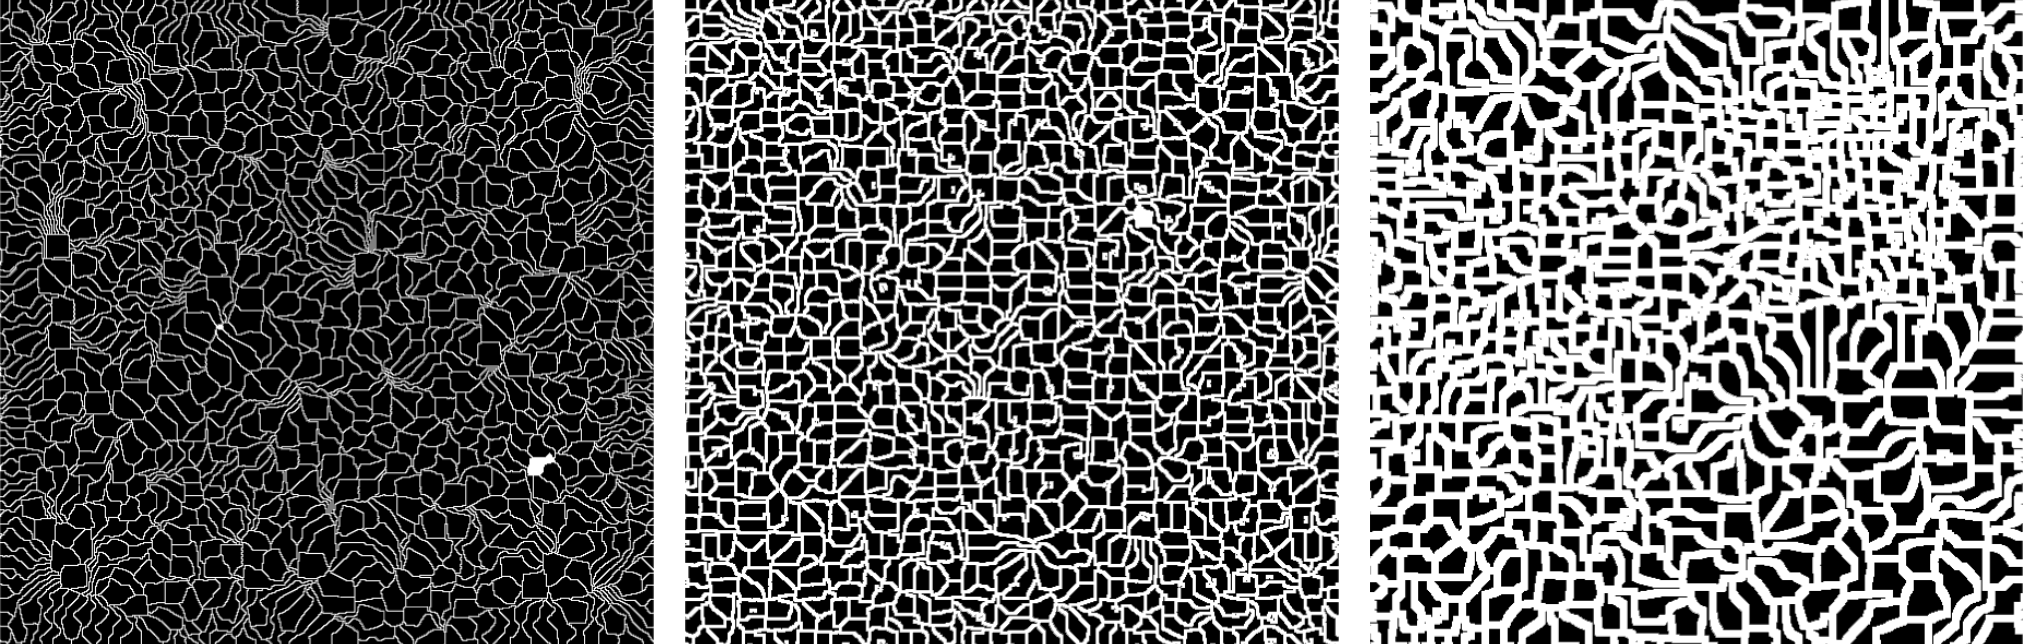
\includegraphics[width=13cm]{sistdin1}}
  \caption{Diferentes separaciones entre part\'iculas utilizando el par\'ametro separación. Izquierda: separaci\'on = 1, centro: separaci\'on = 2, derecha: separaci\'on = 4.}
  \label{fg:sistdin1}
\end{figure*}

Finalmente, el algoritmo devuelve la grilla $L$, la cual ser\'a renderizada posteriormente. En la siguiente secci\'on se explica la utilizaci\'on de sistemas din\'amicos en la evoluci\'on guiada de part\'iculas.

\subsection{Sistemas Din\'amicos}

Las ecuaciones diferenciales tienen como prop\'osito tratar con la dificultad (o imposibilidad) de hallar soluciones anal\'iticas en procesos din\'amicos. En primer lugar, se define un modelo matem\'atico del problema, del cual luego se obtienen 
las ecuaciones diferenciales asociadas. Los mismos se resuelven por medio de aproximaciones num\'ericas en cada instante de tiempo.

Los costos computacionales de estas soluciones dependen de la complejidad del problema y el n\'umero de ecuaciones del sistema. En este trabajo proponemos utilizar una sub-\'area de ecuaciones diferenciales llamada ecuaciones diferenciales ordinarias (ODE). En esta representaci\'on, el tiempo es tratado como la \'unica variable independiente.


De manera general, las ODEs se representan utilizando el siguiente sistema de ecuaciones:
\begin{equation} \label{eq:simple}  
  \begin{aligned}
    \dot{x_{1}} = f_{1}(x_{1},\ldots,x_{n}),\\
    \ldots\\
    \dot{x_{n}} = f_{n}(x_{1},\ldots,x_{n}),
  \end{aligned}
\end{equation}

\noindent donde $\dot{x_{i}}$ representa la derivada de $x_{i}$ con respecto
a $t$. Las variables $x_{i}$ y las funciones $f_{i}$ se definen de manera diferente para cada problema. En este caso, cada variable representa una coordenada cartesiana en el espacio, $x_{1}$ es $x$, $x_{2}$ es $y$ y $x_{3}$ es $z$. El conjunto de $f_{i}$ ser\'a definido tratando de capturar la estructura interna del pan. La siguiente secci\'on muestra cómo estos sistemas pueden describir la evoluci\'on de los sistemas de part\'iculas.

\subsection{Evoluci\'on de sistemas de part\'iculas utilizando sistemas din\'amicos}

La percepci\'on humana puede detectar patrones en la estructura de la miga de pan. Distintas observaciones pueden realizarse sobre la distribuci\'on de las burbujas en la misma (ver Fig.~\ref{fg:panreal}). Primero, la forma de las burbujas cercanas a la corteza tiende a estirarse paralelamente a la misma. Esto es resultado de la acci\'on de las elevadas temperaturas durante la cocci\'on de la masa. Tambi\'en resulta evidente que la estructura completa es similar a un fluido con la forma de la corteza.


\begin{figure*}[htb!]
  \centerline{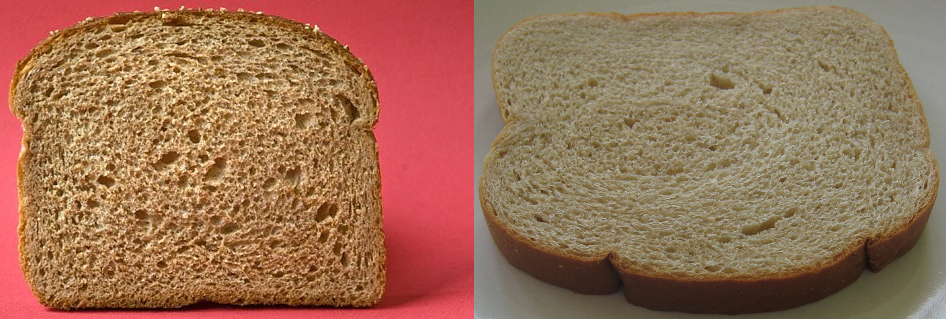
\includegraphics[width=13cm]{panreal}}
  \caption{Im\'agenes de cortes reales de pan}
  \label{fg:panreal}
\end{figure*}

Por otro lado, los sistemas din\'amicos previamente presentados producen formas naturales (ver Fig.~\ref{fg:sistdin2}). En las im\'agenes pueden observarse c\'irculos y espirales, entre otras formas. Las im\'agenes se obtuvieron dibujando trayectorias sobre un plano, siguiendo distintas ODEs. Tres ODEs describen las din\'amicas presentes en las im\'agenes. A modo de ejemplo, la imagen de la izquierda es el resultado del siguiente conjunto de ecuaciones:

\begin{equation} \label{eq:simple}  
  \begin{aligned}
    \dot{x} &= x^{2}-y^{2}+1,\\
    \dot{y} &= 2xy+1.
  \end{aligned}
\end{equation}


\begin{figure*}[htb!]
  \centerline{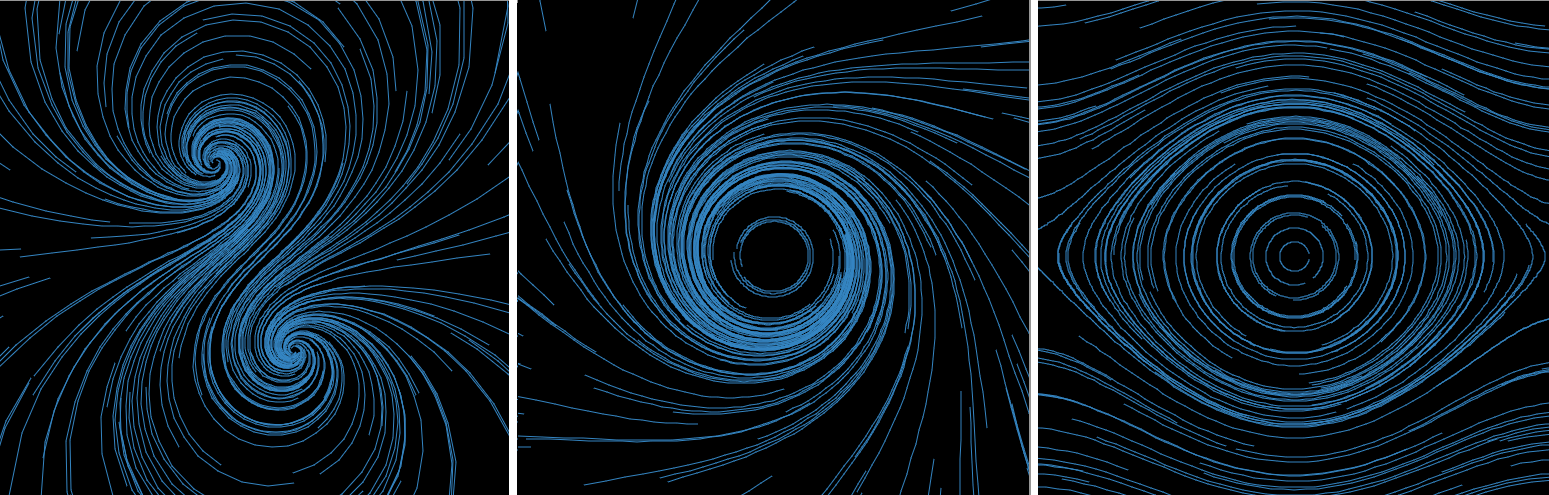
\includegraphics[width=13cm]{sistdin2}}
  \caption{Sistemas din\'amicos en el plano.}
  \label{fg:sistdin2}
\end{figure*}

En los ejemplos se eligen posiciones aleatorias y luego el sistema se resuelve por medio de un {\em solver} Runge-Kutta de cuarto orden, el cual permite conocer la direcci\'on a tomar en cada punto por la trayectoria (en las im\'agenes se computaron trayectorias hacia adelante y hacia atrás en el tiempo para lograr una mejor visualizaci\'on). La imagen de la izquierda muestra un atractor y un repeledor claramente visibles. El centro de la espiral m\'as a la izquierda es un atractor (a medida que $t$ avanza, las trayectorias convergen hacia el punto), mientras que el otro centro es un repeledor. Los atractores pueden no ser puntuales, como muestran las restantes dos im\'agenes. La imagen de la derecha muestra atractores en forma de c\'irculos (las trayectorias ciclan por el c\'irculo).

Las part\'iculas producen distintos patrones al seguir las trayectorias definidas en el plano y el espacio. Esto se logra resolviendo num\'ericamente el sistema din\'amico en la posici\'on agregada a la part\'icula, seleccionando como siguiente posici\'on de crecimiento aquella posici\'on del contorno que mejor aproxima la soluci\'on del sistema din\'amico (para esto, sólo se agrega al contorno esa posición). El Algoritmo $2$ muestra cómo se modifica el algoritmo de modelado para incluir este comportamiento.

\begin{algorithm}[h!]
\caption{Modificación del algoritmo de modelado por medio de sistemas dinámicos}
\begin{algorithmic}
\State $L[h]\gets 0$ \Comment{masa $\rightarrow$ aire}
\State $O[i].agregar(h)$
\State $solucion \gets Runge\_Kutta(h)$
\Comment {Se calcula la siguiente posición}
\State $vec = vecindario(h)$
\State $mejor = abs(vec[0] - solucion)$
\State $elegida = h$
\State $vec.eliminar(h)$
\For {$w \in vec$}
\State{// Se calcula la posición del vecindario que mejor aproxima al sistema}
    \If {$abs(vec[w]-solucion) < mejor$}
        \State $mejor = abs(vec[w]-solucion)$
        \State $elegida = w$
    \EndIf
    \If {$aleatorio() > 1-aleatoriedad$} 
    \Comment {$0 <= aleatorio() <= 1$}
        \State $C[i].agregar(w)$
    \EndIf
\EndFor
\State{// Se agrega al vecindario sólo la posición que mejor aproxima la solución}
\State $C[i].agregar(elegida)$
\end{algorithmic}
\end{algorithm}

Las part\'iculas se deforman de forma global en un patr\'on que es visualmente similar a las trayectorias que produce el sistema (ver Fig.~\ref{fg:sistdin3}). En las im\'agenes, de izquierda a derecha se decrementa la {\em aleatoriedad} de las trayectorias. El par\'ametro aleatoriedad seteado a $0.1$ genera la imagen de la derecha, lo cual significa que las burbujas eligen como siguiente posición de crecimiento la que mejor se acopla al sistema con una probabilidad de $0.9$. La probabilidad se define como $1-aleatoriedad$, donde $0 \leq aleatoriedad \leq 1$. Las ecuaciones del sistema son las mismas que las de la imagen derecha mostrada en la Fig.~\ref{fg:sistdin2}. Estos patrones pueden ser utilizados adem\'as en otros materiales cocidos, variando el par\'ametro de aleatoriedad. Distintos sistemas de ecuaciones pueden utilizarse para definir distintos patrones.

\begin{figure*}[htb!]
  \centerline{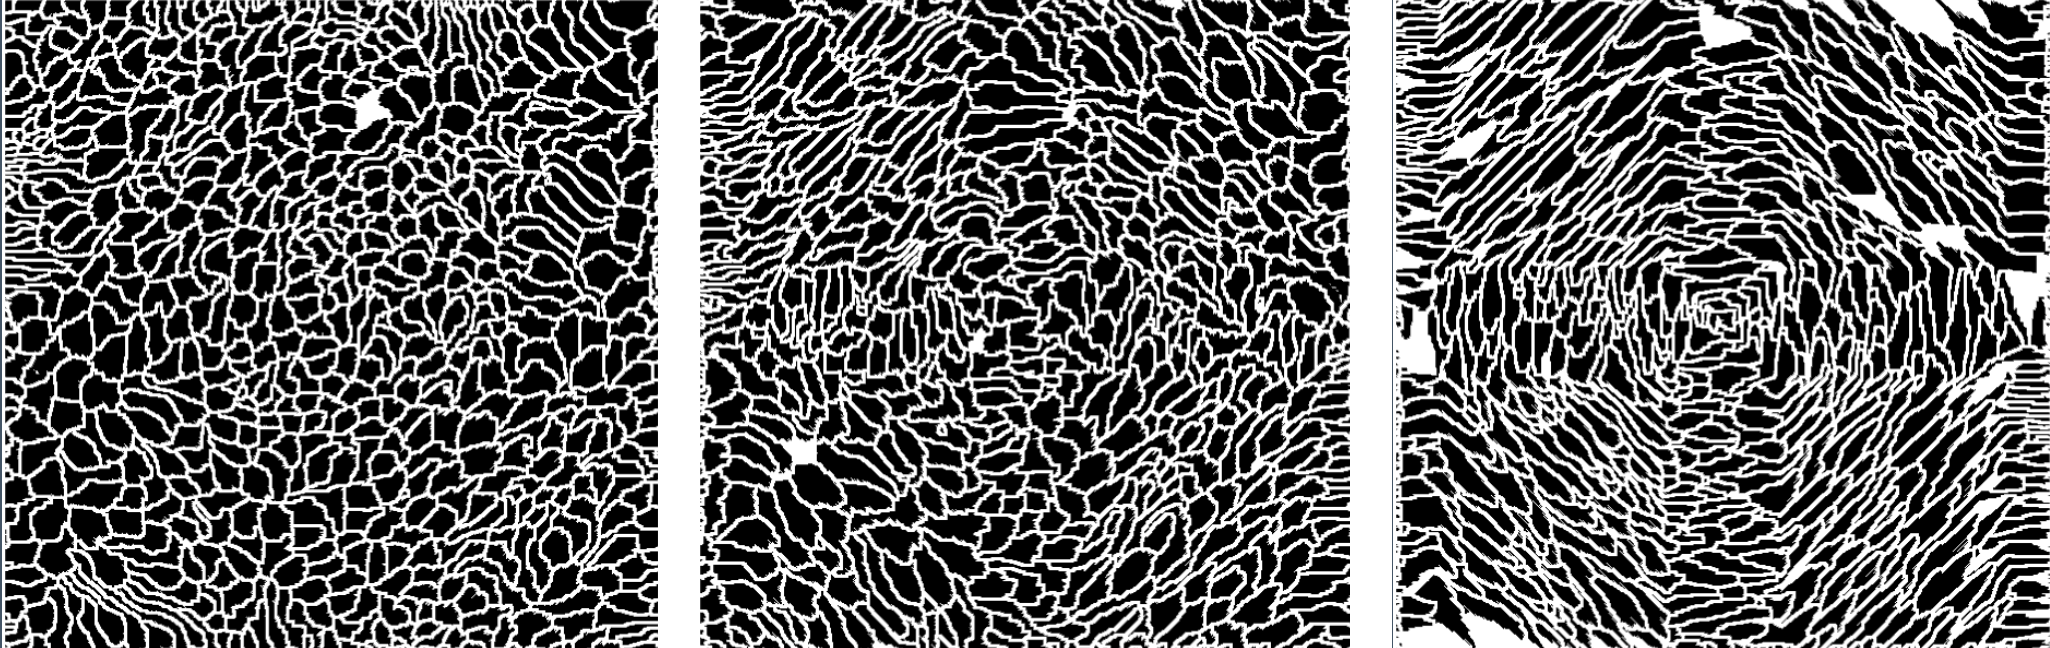
\includegraphics[width=13cm]{sistdin3}}
  \caption{Sistemas din\'amicos aplicados en sistemas de part\'iculas. Efecto del parámetro {\em aleatoriedad}. De izquierda a derecha, aleatoriedad: 0.3,0.2,0.1 respectivamente. }
  \label{fg:sistdin3}
\end{figure*}

\subsection{Resultados y Limitaciones}
Las Figs.~\ref{fg:crumb} y \ref{fg:results2} muestran imágenes renderizadas utilizando el procedimiento descrito.

\begin{figure}
  \centerline{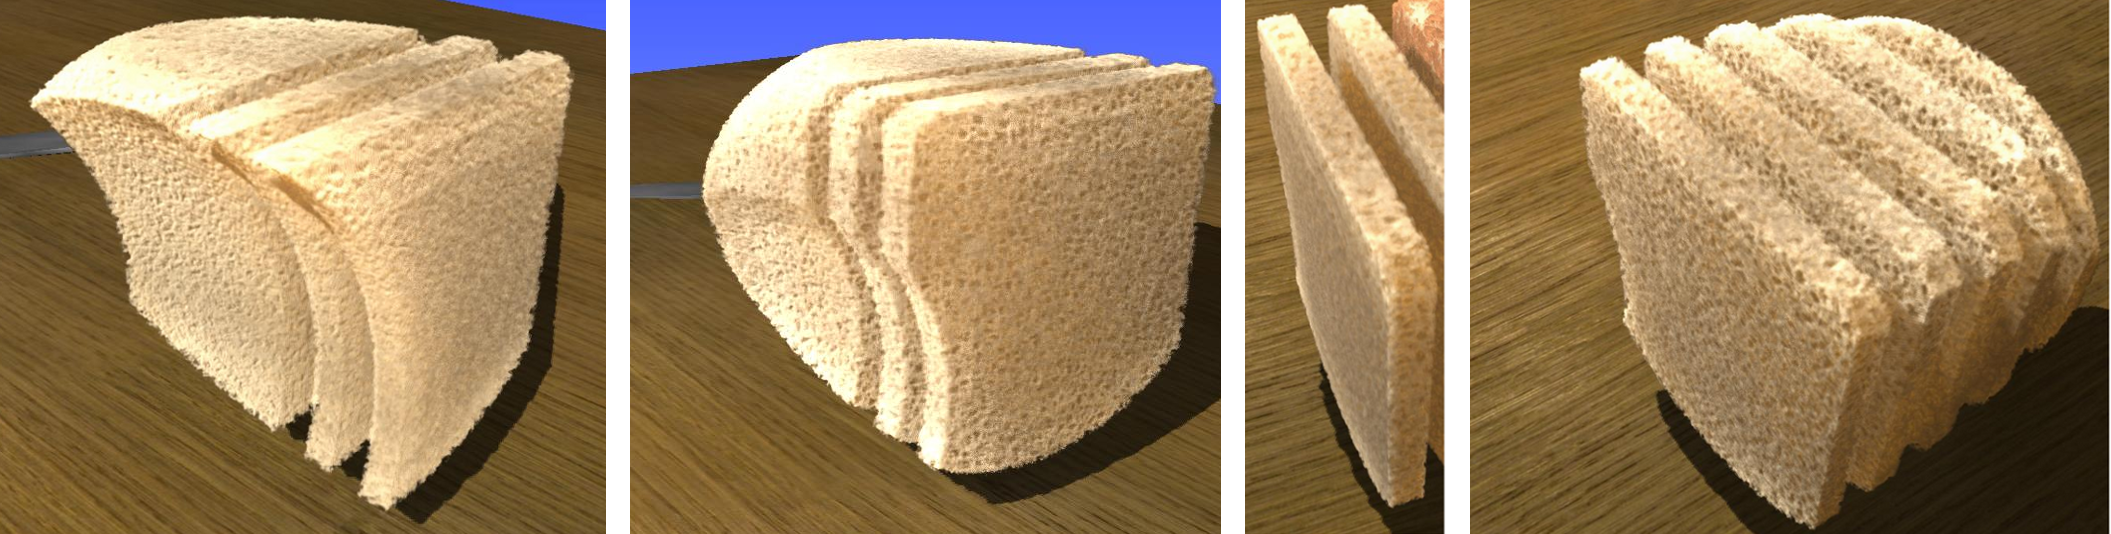
\includegraphics[width=13cm]{figures/crumb}}
  \caption{Miga de pan sintetizada, vista desde distintos ángulos.}
  \label{fg:crumb}
\end{figure}


\begin{figure}
  \centerline{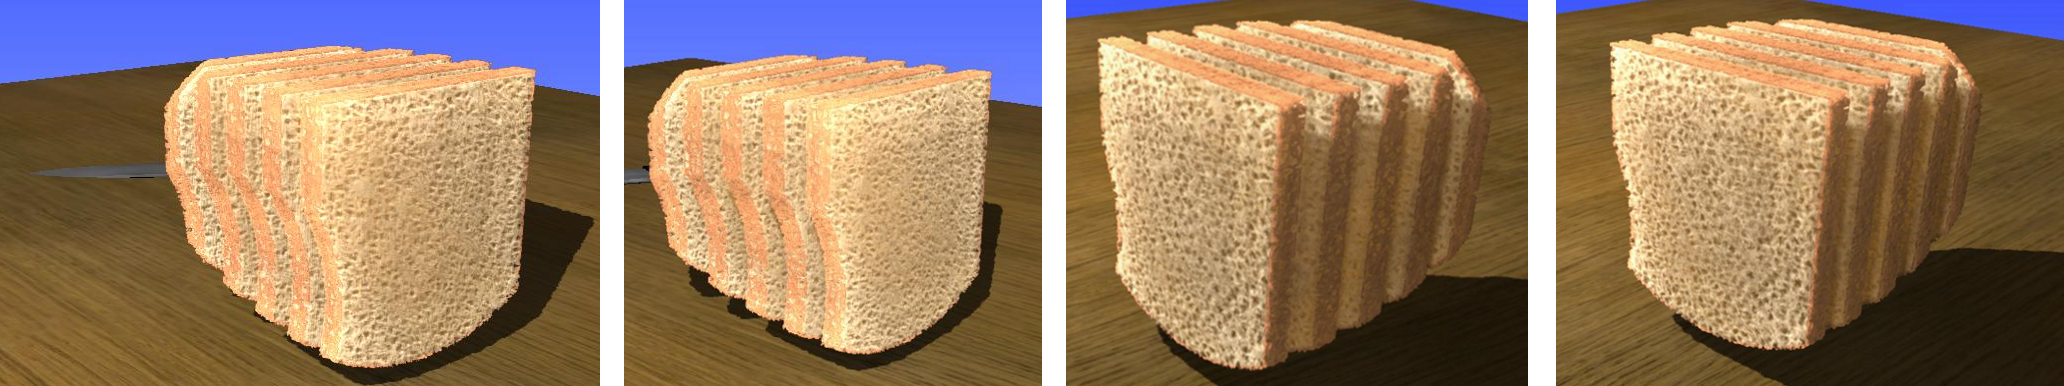
\includegraphics[width=13cm]{figures/results2}}
  \caption{Miga de pan sintetizada, vista desde distintos ángulos (con corteza agregada).}
  \label{fg:results2}
\end{figure}

Si bien es posible la obtención de distintas geometrías de manera sencilla y prácticamente de manera automática, todavía existen limitaciones en cuanto a la flexibilidad de los tipos de pan a producir.
Se depende de un sistema dinámico para producir la forma global de la deformación, pero este sistema es difícil de controlar.
Además, no siempre se adapta de manera sencilla a la forma exterior del material.
Debido a esto, en la siguiente sección presentamos un algoritmo más robusto el cual permite superar estas deficiencias.
El mismo continúa con la idea de la utilización de una definición volumétrica del material, pero el mismo está basado en modelos físicos del proceso de fabricado del pan, extraído directamente de la literatura de ingeniería de los alimentos.

\section{Modelado del Pan desde su Proceso de Fabricación}
Para lograr un modelado realista de la geometría de la miga de pan es necesario comprender su proceso físico de formación.

\begin{figure*}
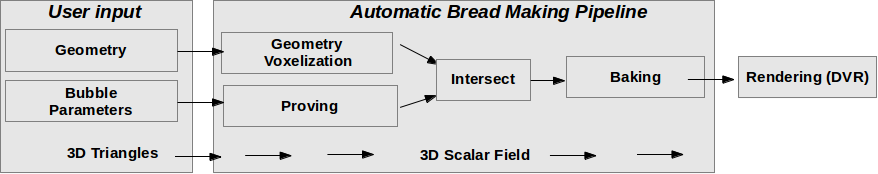
\includegraphics[width=13cm]{figures/pipeline}
\caption{Procedimiento semi-automático para obtener pan sintético foto-realista}
\label{FigPipeline}
\end{figure*}

Utilizando las ideas de la sección anterior, proponemos otro modelo volumétrico de generación de geometrías de migas de pan.
En esta sección proponemos unificar, y diferenciar, los pasos claves presentes en el proceso de fabricación del pan (sobre todo, leudado y cocción).
El procedimiento busca utilizar el proceso físico de generación de geometrías de migas y cortezas de pan a partir de la masa original.
Estos procesos han sido vagamente tenidos en cuenta en la literatura, la cual ha atendido siempre a procesos artísticos más simples, dada la complejidad de los mismos.

En primer lugar, reveeremos el estado del arte del proceso de fabricación del pan.
% e introduciremos modelos matemáticos requeridos para comprender el proceso de cocción.
Luego presentaremos los procesos de modelado, que junto con el modelo de iluminación del siguiente capítulo, permiten obtener imágenes foto realistas de distintos tipos de pan.

\subsection{Trabajo Previo}
El modelado procedimental de geometría reduce fuertemente la necesidad de intervención artística en dominios o situaciones donde la utilización de supervisión repetitiva del proceso se torna impráctica, por ejemplo al modelar ciudades \cite{Parish2001}, planetas \cite{Ebert2002}, edificios \cite{Muller2006}, y plantas \cite{Prusinkiewicz1990}. 
Algunos métodos procedimentales utilizan gramáticas para definir descripciones matemáticas, representando relaciones espaciales entre las primitivas, por ejemplo cubos, cilindros o líneas.
Las estructuras finales usualmente emergen utilizando recursión sobre elementos gramaticales.

Si bien existen algunos ejemplos en la literatura sobre modelado y renderizado de la estructura de migas de pan \cite{Tong2005,Xenakis2007}, los mismos ignoran casi por completo el proceso real de formación.
Algunos trabajos pioneros aplicaron modelos físicos de cocción a determinados tipos de pan para su renderizado, buscando obtener animaciones ({\em e.g.} \cite{Rodriguez-Arenas2011}), pero el modelado de la geometría de las burbujas de la miga del pan no fue tenido en cuenta.

Por otro lado, el modelado procedimental de panes es un tópico multidisciplinario de investigación.
La ingeniería de los alimentos lleva varias décadas de publicaciones en el área, tratando de desarrollar un mejor entendimiento del proceso de formación del pan.
Esta rama de la ciencia muestra que el leudado determina fuertemente las características presentes en la miga de pan, particularmente las burbujas \cite{Babin2006}.
La interacción entre la levadura y algunos nutrientes presentes en la masa produce {\em $CO_{2}$}. 
El radio de las burbujas y sus distribuciones espaciales muestran estructuras con características fractales, exhibiendo autosimilaridad estadística en diferentes escalas de medición.
Determinados trabajos han computado las dimensiones fractales de estas estructuras en determinados tipos de pan \cite{Gonzales2008}, sugiriendo distribuciones fractales uniformes.
El modelado de la cocción del pan es sujeto de numerosos trabajos \cite{Mondal2008}.

El modelado procedimental utilizando fractales también atendió las necesidades de otros variados materiales como montañas \cite{Prusinkiewicz1993}, cráteres lunares, y distribución de las burbujas en quesos \cite{Mandelbrot1983}. 
Adicionalmente, determinados modelos matemáticos complejos representan el comportamiento y el crecimiento de diversos fenómenos naturales.
En computación gráfica, estos modelos son unas de las fundaciones usadas para modelar agua y fluidos \cite{Stam1999,Fedkiw2001}.
Estos trabajos utilizan complejos modelos diferenciales de otras ramas de la ciencia y las aproximan con técnicas numéricas.
En años recientes, la tecnología GPGPU \cite{Owens2007} permitió la posibilidad de alcanzar tiempos reales o interactivos en el cómputo y renderizado de estos modelos numéricos.

A pesar de todos estos avances, el modelado y visualización foto-realista de panes y materiales porosos todavía presenta diversos retos.
Además de un modelo geométrico realista, el renderizado requiere que se represente de manera adecuada los fenómenos de transporte de la luz, incluyendo auto-oclusión, auto-sombreado, transmitancia, translucencia, transparencia, entre otras.
Solamente unas pocas publicaciones proponen atacar ambos problemas, pero utilizando consideraciones artísticas \cite{Xenakis2007}.
Además, estos autores no dan suficientes detalles del modelado y renderización ya que existen derechos de propiedad intelectual, limitando enormemente la reproducción de dichas imágenes.

Por otro lado, la comunidad artística usualmente produce imágenes realistas de pan utilizando fotografías de los mismos, y definiendo geometrías a partir de ellas, junto a la utilización de materiales translúcidos\footnote{http://www.blenderguru.com/tutorials/how-to-create-realistic-bread} y otras consideraciones {\em ad-hoc}\footnote{http://design.tutsplus.com/tutorials/create-a-realistic-loaf-of-bread-in-photoshop--psd-10555}.
Si bien los resultados obtenidos son buenos, los procesos son tediosos y demandan horas.
Además, si se requiere más de una imagen, es necesario repetir todo el proceso desde el principio, lo que torna al mismo muy poco práctico.
Existen numerosas desventajas además de esta.
Por ejemplo, no es posible obtener cortes arbitrarios del material resultante.


\subsection{Visión global del Proceso}
La Fig.~\ref{FigPipeline} muestra el proceso completo de formación de geometrías sintéticas de pan.
Todos los pasos se aplican sobre campos escalares.
Los usuarios pueden proveer el sistema con un modelo de tres dimensiones de su preferencia, o dejar que el sistema provea un pan de forma estándar ({\em croissants}, {\em baguettes}, etc.).
La geometría introducida se voxeliza para proceder a las siguientes etapas.
En la simulación del proceso de leudado, el usuario puede parametrizar la textura del pan (cantidad y tamaño de las burbujas y su distribución), o nuevamente dejar que el sistema provea parámetros estándar que producen tipos de pan conocidos.
La masa cruda será intersectada con la geometría voxelizada para obtener un campo escalar, el cual tiene la forma externa que provee el usuario (o el sistema), con el interior de la misma compuesta de las burbujas procedentes de los parámetros establecidos (ver Sección~\ref{breadprov}).
Luego, se computa un modelo de cocción específico \cite{Powathil2004} para deformar el campo escalar (y las burbujas de éste), de acuerdo a los efectos que produce la cocción en el proceso de formación del pan.
El último paso aplica renderizado directo de volúmenes (direct volume rendering, DVR) \cite{Kruger2003} al campo escalar resultado de la cocción, obteniendo imágenes realistas del pan resultante.

%====================================================================

\subsection{Voxelización de la Geometría}

En nuestro modelo es posible generar panes con geometrías arbitrarias, supliendo un modelo de triángulos en algún formato estándar.
El modelo consta de un conjunto de pasos. El primer paso de la secuencia voxeliza un modelo provisto por un usuario con la utilidad de código abierto {\tt binvox} \footnote{http://www.cs.princeton.edu/~min/binvox/} \cite{Nooruddin2003}.
La voxelización genera un campo escalar binario, con $1$ representando que el voxel dado está dentro de la geometría, y $0$ significando que el voxel está fuera de la geometría.
El paso de leudado (siguiente subsección) genera la textura del material que se ubica dentro de esta geometría voxelizada.
Esto permite generar panes con formas arbitrarias, tales como {\em baguettes}, {\em croissants}, {\em lactal}, u otros menos comunes (una tetera o un conejo).

Un sub-producto importante de la matriz de geometría es un campo escalar secundario que puede ser obtenido por medio de una transformación de distancia.
La transformación de distancia genera una matriz $n$-dimensional con las mismas dimensiones que la matriz que se transforma \cite{osh03}.
La transformación computa, para cada entrada distinta de cero en la matriz, la distancia más cercana a una entrada nula de dicha matriz.
Dada una matríz $n$-dimensional $M$, el algoritmo genera una matriz a valores reales $DF_{M}[i]$ con las mismas dimensiones que $M$,


$$  DF_{M}[i] = \min \bigg\{ \delta(i,j): M[j] = 0 \bigg\},$$

%\begin{align*}
%M'[i] &= min(d(i,j)), M[i] != 0, M[j] = 0\\
%M'[i] &= 0, M[i] = 0,
%\end{align*}

\noindent
donde $\delta(i,j)$ podría ser la distancia de Manhattan o la distancia Euclideana en un espacio $n$ dimensional.
Las entradas de la matriz lejanas a los bordes del objeto tomar valores más altos que aquellas cercanas a los mismos.
De esta manera se obtiene un mapa de la distancia de cada voxel a las superficies tridimensionales del objeto.
Este campo escalar de distancias será requerido en etapas posteriores del proceso.


\subsection{Simulación del Leudado}
\label{breadprov}
Como fue establecido, la textura observable en la masa cruda del pan está compuesta de burbujas, cuya distribución exacta es el resultado de procesos complejos, entre ellos, reacciones químicas, y deformaciones físicas de la masa.
El paso de leudado consta en primera instancia del crecimiento libre de las burbujas, producido por seres vivos, la levadura.
Luego, el cocinero interviene la masa deformándola de diversas maneras.
Finalmente el paso de cocción produce la textura y distribución de burbujas finales.
Los estudios fenomenológicos de estas texturas utilizan tomografía de rayos X y extracción de características sobre las mismas \cite{Gonzales2008,Babin2006,VanDyck2014}.
Buscando obtener una variabilidad similar, en esta tesis generamos distribuciones de burbujas con un modelo basado en fractales, inspirado en las distribuciones de burbujas presentes en el queso, y la textura inducida por los cráteres lunares, propuesto en \cite{Mandelbrot1983}.
Luego validamos los mismos utilizando el método multifractal denominado {\em Sandbox} (caja de arena, ya que realiza cálculos sobre una distribución de puntos aleatoria en la geometría).
Esto será explicado en profundidad en el capítulo de validación.

La textura de la masa es creada procedimentalmente en un campo escalar separado, definido en una matriz de tres dimensiones, de una manera similar a la matriz de geometría en la Subsección arriba.
Cada voxel es iniciado a $1$ (significando que el material aún no tiene burbujas).
El proceso comienza substrayendo esferas de radio $r_{min}$ posicionadas arbitrariamente en el campo escalar (esto se logra seteando a $0$ las celdas respectivas).
Luego, substraemos esferas de radio mayor, nuevamente en posiciones arbitrarias, hasta un radio máximo $r_{max}$.
La relación entre el número de esferas $N_{s}$ a ser sustraídas en cada paso, y sus respectivos radios $r$, está dada por la ley fractal,


\begin{equation*}
N_{s} = \frac{k}{r^{d}},
\end{equation*}

donde $d$ es el exponente fractal que modela la ocurrencia de esferas en relación con su radio, y $k$ controla la cantidad de esferas para cada radio.
Con estos simples parámetros basta para modelar una gran cantidad de texturas en general, particularmente pan.

La Fig.~\ref{FigProving} muestra un ejemplo de un corte en dos dimensiones de este modelo.
Si bien las burbujas esféricas resultantes no son completamente realísticas debido a su forma, los resultados muestran un notorio parecido en tamaños y distribución de tamaños con binarizaciones de cortes reales de masas leudadas (ver \cite{Babin2006}).
Durante la cocción, el campo escalar resultante será sometido a deformaciones geométricas. Consecuentemente, la textura final se ajustará aún más a burbujas de panes reales.
Finalmente, en la sección de validación se buscarán parámetros de generación que ajusten diferentes panes reales. 

\begin{figure}
\center
\includegraphics[width=7cm]{figures/bubbles}
\caption{Simulación Fractal del Leudado de Pan.}
\label{FigProving}
\end{figure}

Luego de la voxelización y la simulación de leudado, las burbujas deben estar presentes sólo en el interior de la geometría.
Para esto, intersectamos ambos campos escalares utilizando un simple producto punto a punto, es decir, una máscara,

\begin{equation*}
P_{2} = P_{1} * G,
\end{equation*}
%
donde $P_{1}$ es el campo $3D$ (matriz) que contiene las burbujas del leudado, y $G$ es el campo escalar que representa a la geometría voxelizada.

La Fig.~\ref{fg:intersectProblem} muestra una versión renderizada de esta intersección.

\begin{figure*}
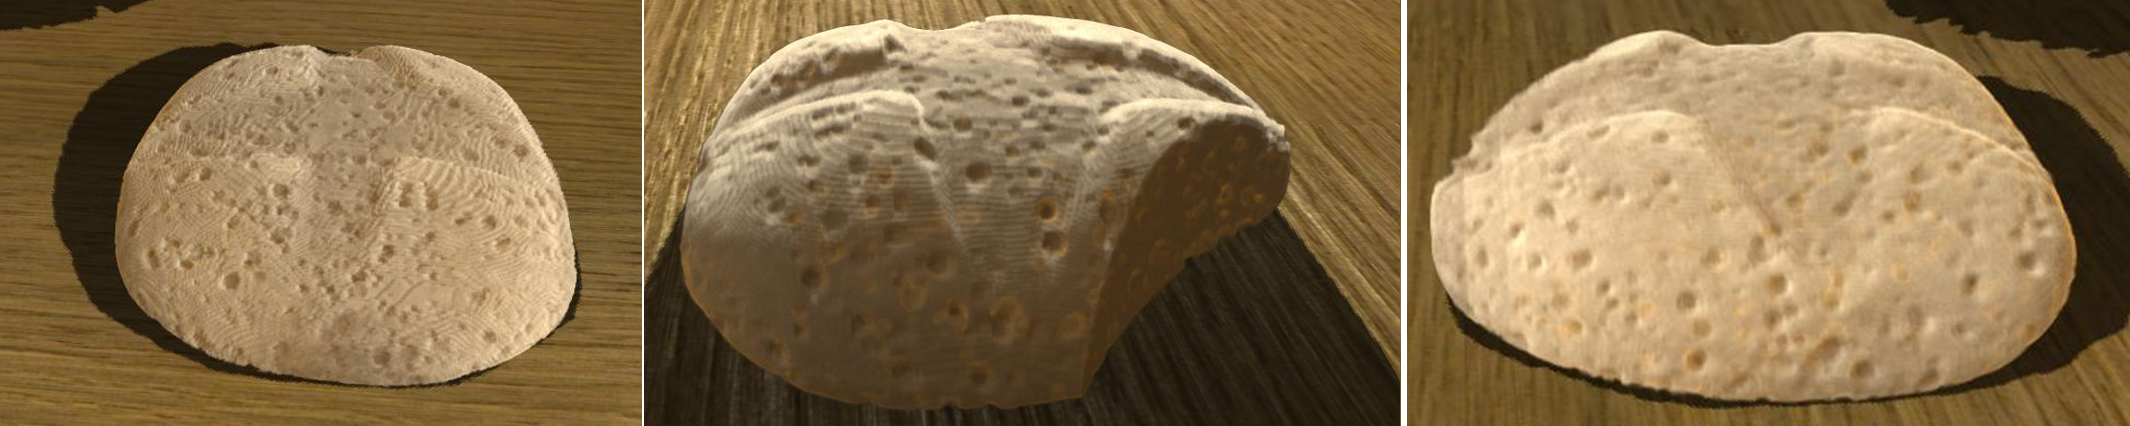
\includegraphics[width=13cm]{figures/intersectProblem}
\caption{Intersección simple de la geometría y de las burbujas provenientes del leudado. A diferencia de masas reales, pueden verse burbujas en la superficie de la masa.}
\label{fg:intersectProblem}
\end{figure*}

Si bien los resultados pueden parecer realistas, en panes reales, no es habitual que las burbujas sean visibles en la superficie, debido al leudado y cocción reales.
Para solucionar este problema, utilizamos el campo escalar de distancias que computamos previamente, para deshabilitar la generación de burbujas en zonas cercanas a los bordes de la geometría, de acuerdo a cierto valor umbral, el cual será un parámetro.
El campo escalar binario resultante se computa de la siguiente manera,

%\begin{align*}
%DF    &= distField(G),\\
%interior &= DF > umbral,\\
%masa &= G - interior*(1-P_{2}),
%\end{align*}
%
%donde $DF$ es el campo escalar de distancias a la superficie, computado a partir de la geometría de entrada, voxelizada, y $umbral$ es un parámetro que determina el ancho de la región exterior, donde no pueden crearse burbujas.
%Computamos la masa final substrayendo las burbujas ($1-P_{2}$) de la geometría original, pero limitada a la región {\em interior} que acabamos de definir.
Las Figs.~\ref{fg:proving} y \ref{fg:provingBunny} muestran resultados de limitar las interacciones de burbujas a la región interior de la geometría original, donde se observa que no existen burbujas en la superficie de la masa, como ocurre en masas reales.
Las imágenes muestran que el método definido es capaz de producir imágenes realistas de panes crudos con formas arbitrarias.
Cabe remarcar que el modelo es lo suficientemente flexible, permitiendo renderizar el material en cualquier etapa de su proceso de fabricación, además de poder realizar cortes arbitrarios del mismo.

\begin{figure*}
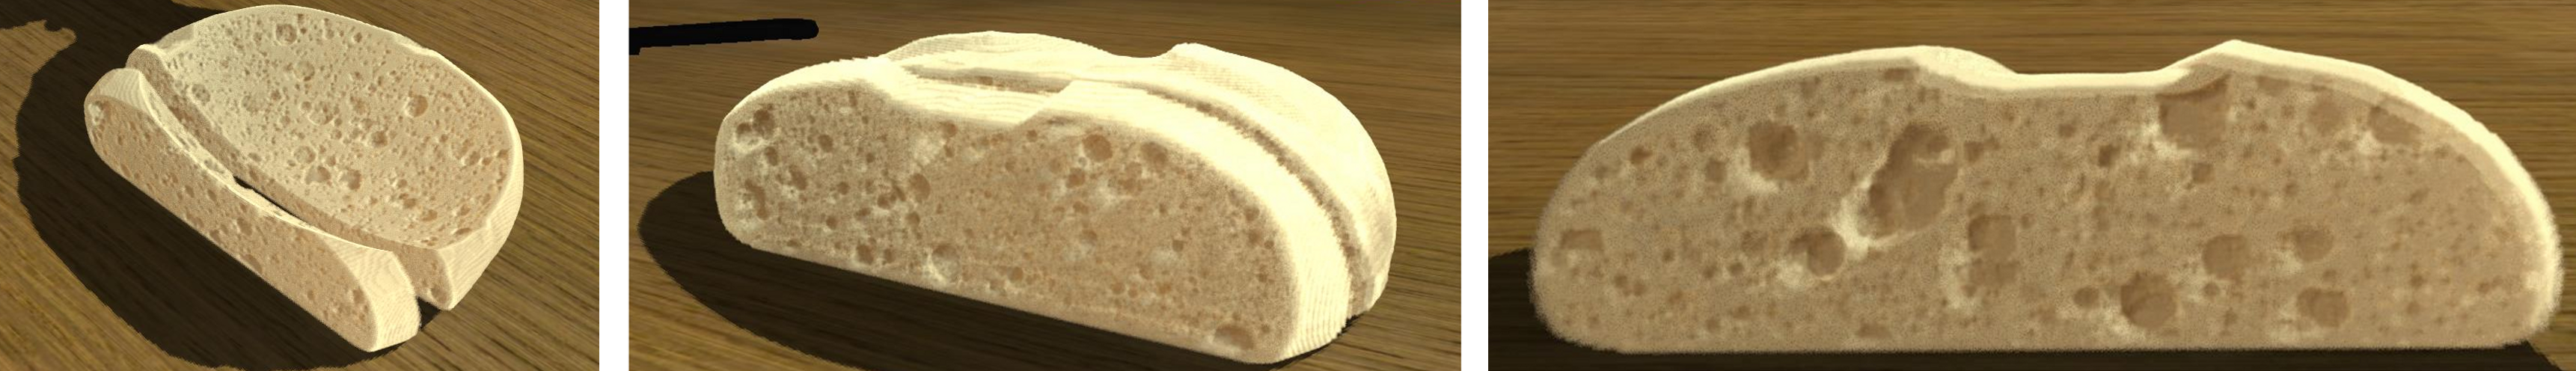
\includegraphics[width=13cm]{figures/prebakebread}
\caption{Pan luego del leudado, y antes de la cocción.}
\label{fg:proving}
\end{figure*}

\begin{figure*}
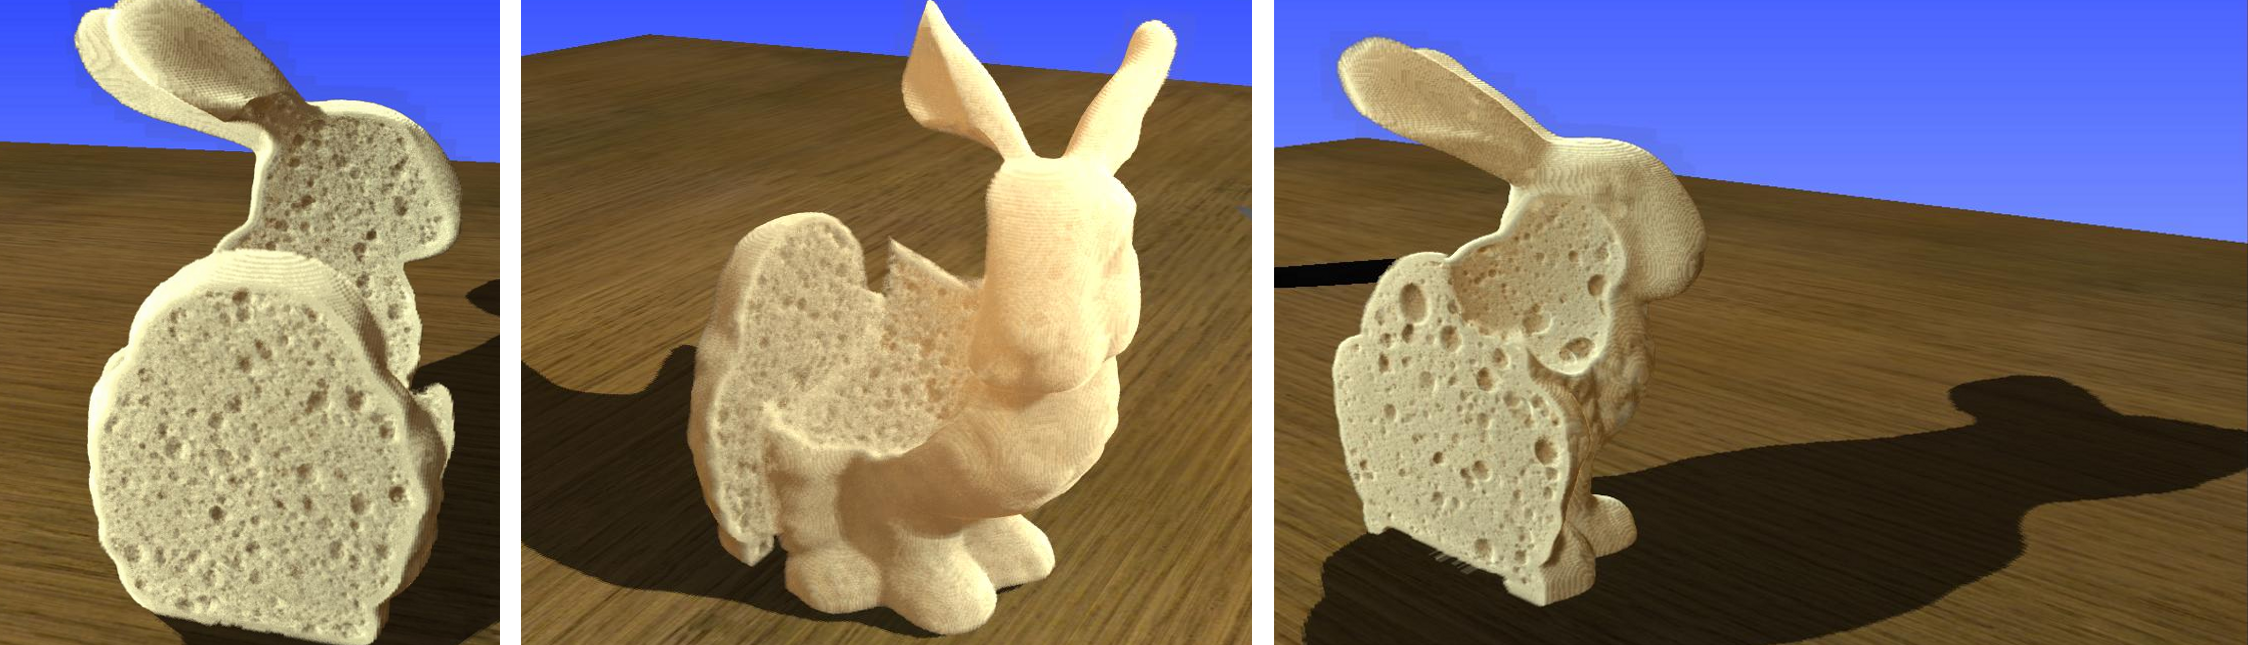
\includegraphics[width=13cm]{figures/prebakebunny}
\caption{Conejo de pan, luego del leudado, y antes de la cocción.}
\label{fg:provingBunny}
\end{figure*}

%====================================================================
\subsection{Cocción}
%To adequately simulate the bread baking process, mathematical models should be able to accurately model the heat and mass transfer in dough.
Los modelos matemáticos del proceso de cocción del pan deben ser capaces de modelar correctamente las transferencias de calor y masa en el mismo.
Los modelos físicos más completos del proceso producen soluciones precisas a la distribución de temperaturas en la masa durante la cocción.
Sin embargo, estos modelos son usualmente muy complejos para implementar y son muy costosos computacionalmente.
Además, sólo los modelos más complejos toman en consideración la formación de la corteza del pan.
La corteza, por otro lado, aún carece de una definición formal~\cite{Vanin2009}.
Por lo tanto, los modelos antes citados incluyen sólo una simplificación de la formación de la misma, muy lejos de lo que ocurre en la cocción real.

Los resultados más relevantes en la literatura sugieren que un modelo unidimensional de la cocción puede ser suficiente para la mayoría de los casos prácticos.
Por ejemplo, Purlis~\cite{Purlis2011} modela la cocción del pan como un problema unidimensional, representando la geometría como un cilindro infinito.
Otros trabajos asumen sólo una coordenada radial, resultando también en modelos $1D$~\cite{Powathil2004, Thorvaldsson1999}.
Estos trabajos muestran que utilizar una representación de una única dimensión produce resultados casi idénticos a aquellos que se obtienen utilizando un mayor número de dimensiones, ya que el efecto de la cocción en las burbujas es la menos importante en el proceso de fabricación del pan.

La simulación numérica que implementamos está basada en el esquema de diferencias finitas propuesto por Powathil~\cite{Powathil2004}, y Thorvaldsson y Janestead~\cite{Thorvaldsson1999}. 
El sistema presentado consiste de un conjunto de tres ecuaciones acopladas que describen transferencia de calor, difusión de varpor de agua y difusión de agua líquida.
En nuestro algoritmo, sólo utilizamos las temperaturas ($T$) como entrada para las siguientes etapas de la formación del pan.
La Ec.~\ref{Eq:heat} modela transferencia de calor en la masa del pan, tomando en consideración el balance de energía y evaporación del agua debido a la temperatura~\cite{Thorvaldsson1999},
%
\begin{equation}
\label{Eq:heat}
\frac{\partial T}{\partial t} = \frac{1}{\rho C_{p}} \frac{\partial}{\partial x} \left ( k \frac{\partial T}{\partial x} \right ) + \frac{\lambda}{C_{p}} \frac{\partial W}{\partial t}+\frac{\lambda W}{ \rho C_{p} }\frac{\partial \rho}{\partial t},
\end{equation}
%
donde $T$ es la temperatura, $x$ es la coordenada radial, $t$ es el tiempo, $C_{p}$ el calor específico, $\rho$ la densidad, $k$ la conductividad térmica, $\lambda$ es el calor latente de la evaporación de agua, y $W(x,t)$ es el contenido de agua líquida. 
Las condiciones iniciales
%
\begin{align*}
T(x,0) &= T_{0}(x), 0\le x \le L/2,
\end{align*}
y las condiciones de borde (continuidad y suavidad) definen el modelo,
\begin{align*}
\left ( \frac{\partial T}{\partial x} \right )_{x=L/2} &= 0 , t > 0 \\
-k \left ( \frac{\partial T}{\partial x} \right )_{x=0} &= h_{r}(T_{r}-T_{s}) + h_{c}(T_{air}-T_{s}) - \lambda \rho D_{w} \left (\frac{\partial W}{\partial x} \right )_{x=0}
\end{align*}
%
donde $h_{r}$ y $h_{c}$ son subtérminos del coeficiente de transferencia de calor ($h = h_{r}+h_{c}$), $T_{air}$, $T_{s}$, $T_{r}$ son temperaturas en el aire circundante, en la superficie del pan, y en la fuente de radiación, respectivamente, $L$ es el alto del pan($x = L/2$ es el centro del pan y $x = 0$ es el contorno del mismo), $D_{w}$ representa la difusividad del agua líquida, y $T_{0}$ la temperatura inicial. 
Las temperaturas están expresadas en Kelvin ($K$). 
El modelo consta de ecuaciones similares para la difusión del vapor de agua ($W$) y difusión de agua líquida ($V$).
Otros detalles del modelo pueden ser consultados en \cite{Thorvaldsson1999}.
En nuestro trabajo, utilizamos este modelo para obtener un mapa de temperaturas al final del proceso de cocción.
Estas temperaturas afectarán posteriormente las formas y tamaños de las burbujas.

La simulación de la cocción define el horno a una temperatura típica (por defecto utilizamos $210^{\circ}C$) y discretiza el tiempo en intervalos $\Delta t = 30s$.
De la simulación se obtiene un arreglo $Temp$, de tamaño $N_{grid}$, compuesto por valores de temperatura.
Por estabilidad numérica, utilizamos $N_{grid}=32$ (como en el trabajo original) e interpolamos las temperaturas para obtener mayores resoluciones ($N_{int}$). 
%Each value represents a dough position after $M$ baking time steps. 

El vector obtenido presenta temperaturas decrecientes de $R = 0$ a $R = L/2$, ya que el centro y el borde del pan poseen la menor y la mayor temperatura, respectivamente, luego de la cocción (el calor fluye desde la corteza hacia el centro del pan). 
Si utilizamos el campo escalar de distancias computado previamente, en conjunto con el vector de temperaturas, podemos mapear distancias a temperaturas.
Esto permite definir temperaturas en el campo escalar de forma compatible a una simulación $3D$.
Basados en estos razonamientos, mapeamos el vector de temperaturas $Temp$ en $3D$ de la siguiente manera,

\begin{equation*}
\displaystyle R(x,y,z) = Temp[ round( DF(x,y,z) ) ], 
\end{equation*}
%
donde $R$ es el campo escalar resultante del mapeo, y $x$, $y$ y $z$ son coordenadas $3D$ en $R$. Cuando $DF(x,y,z) = 0$, la posición actual $3D$ se encuentra en la superficie de la geometría, y $Temp[0]$ se mapea $R(x,y,z)$.
Cuando $DF(x,y,z) > 0$, mapeamos una temperatura menor a $R$, ya que la posición actual se encuentra en el interior de la geometría.
La Fig.~\ref{fg:baking} muestra cortes del resultado de este mapeo ($R$), usando temperaturas resultantes de un tiempo arbitrario de cocción, en los tres planos Cartesianos. 
Las imágenes son casi idénticas a lo que se obtendría con una simulación $3D$~\cite{Purlis2010}.

\begin{figure*}
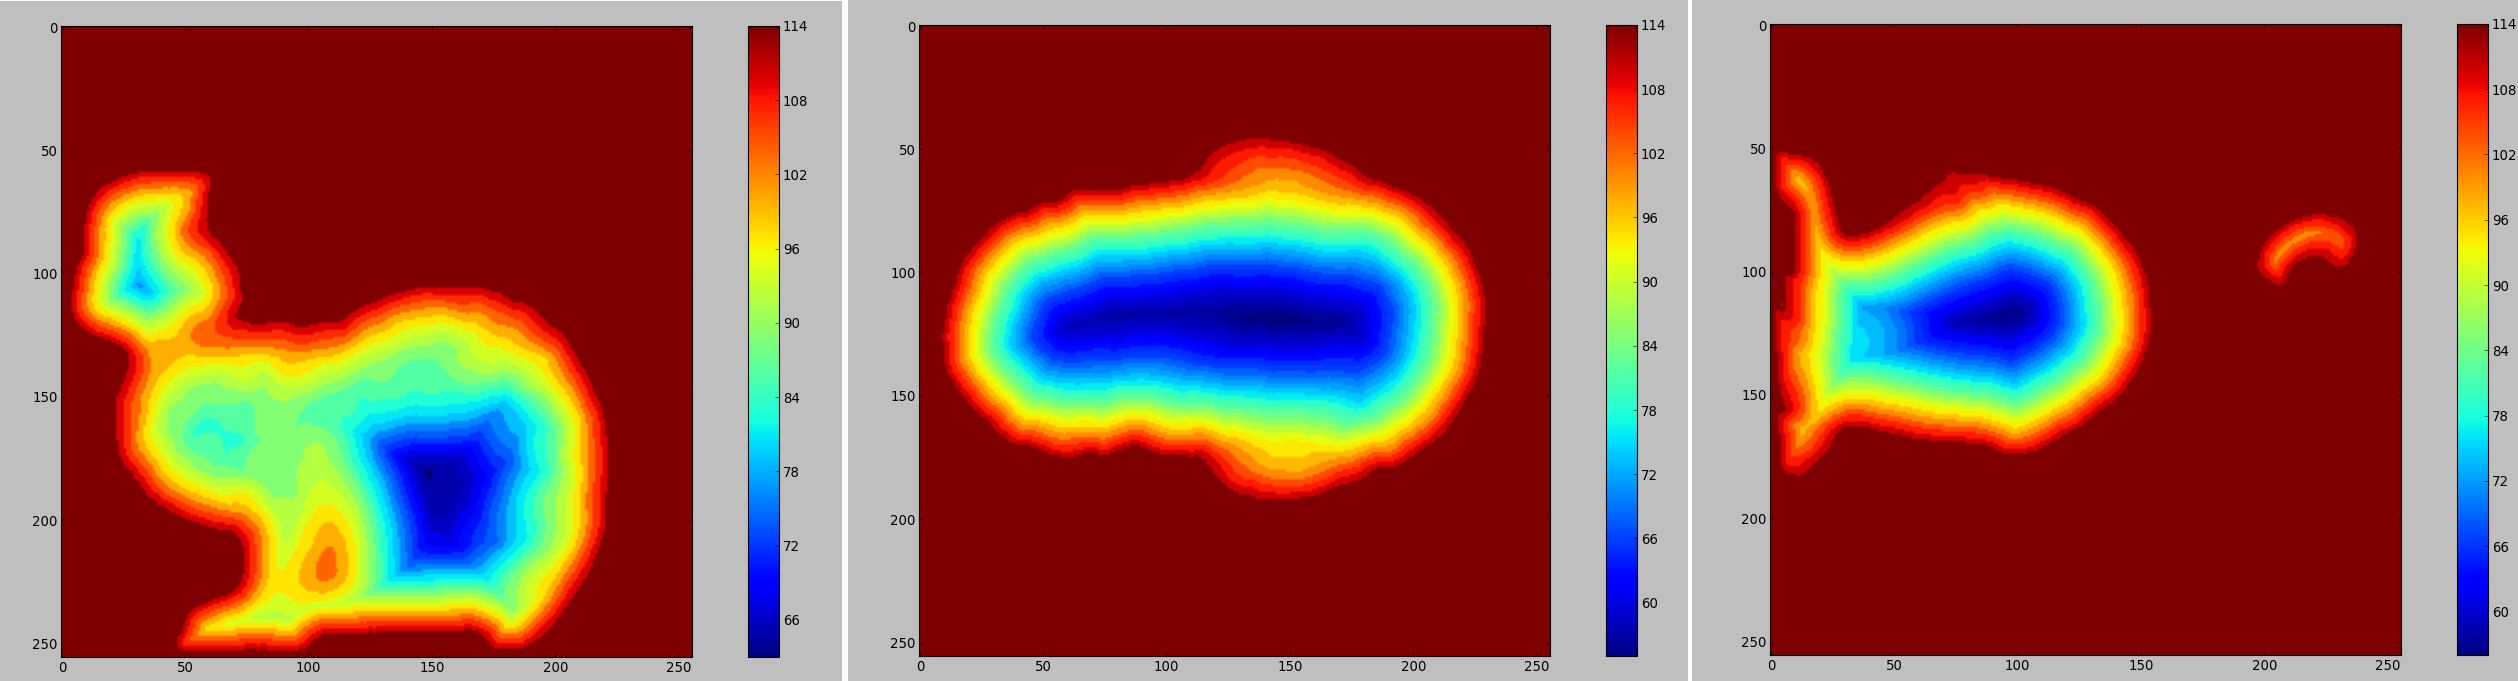
\includegraphics[width=13cm]{figures/tempsbunny}
\caption{Temperaturas unidimensionales mapeadas a un campo escalar con forma de conejo. Las imágenes muestran que la distribución de temperaturas es similar a una simulación en tres dimensiones.}
\label{fg:baking}
\end{figure*}

Luego de cierto número de pasos de simulación ($t=20$ en nuestro caso), computamos el campo vectorial del gradiente ($g$) de $R$ \cite{Gonzalez2006}, y luego suavizamos el mismo utilizando un kernel Gaussiano.
Finalmente, utilizamos las versiones suavizadas para deformar el campo escalar de la siguiente manera,

\begin{align*}
\displaystyle
u &= x+p*g'_{x}[x,y,z],\\
v &= y+p*g'_{y}[x,y,z],\\
w &= z+p*g'_{z}[x,y,z]
\end{align*}
donde $(u,v,w)$ son las coordenadas en el campo escalar resultante, ($x,y,z$) son las coordenadas originales, $p$ es un parámetro real positivo que denota la intensidad con la que se deforma el campo (controla el efecto neto de la cocción en las burbujas), y las $g'$s son las versiones suavizadas del gradiente original $g$.
%Fig.~\ref{FigBakingVectorField} also shows the computed gradient, where using $[-g_{x},-g_{y}]$ produces a similar vector but in the clockwise direction that can be applied with similar effects on the bubbles. 
La Fig.~\ref{fg:bakedbubbles} muestra cortes $2D$ de campos escalares luego de aplicado el proceso de cocción a diferentes formas.

\begin{figure*}
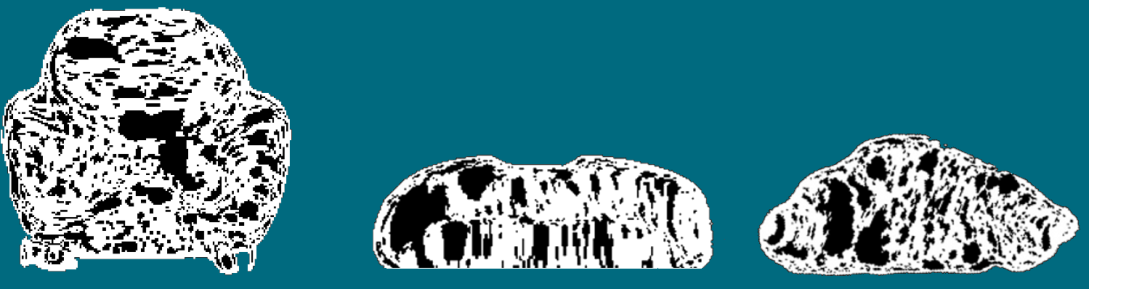
\includegraphics[width=13cm]{figures/bakedbubbles}
\caption{Cortes bidimensionales con burbujas deformadas por el proceso de cocción en diferentes tipos de panes.}
\label{fg:bakedbubbles}
\end{figure*}

El parámetro $p$ puede ser utilizado para sintetizar diferentes apariencias de miga de pan, desde cruda hasta burbujas con mucha deformación (ver Fig.~\ref{fg:parameterp}).
Cuando incrementamos $p$, forzamos a las burbujas a seguir más ajustadamente la forma exterior del pan. 
La imagen también muestra que el método deforma más pronunciadamente las burbujas más cercanas a la corteza.

\begin{figure*}
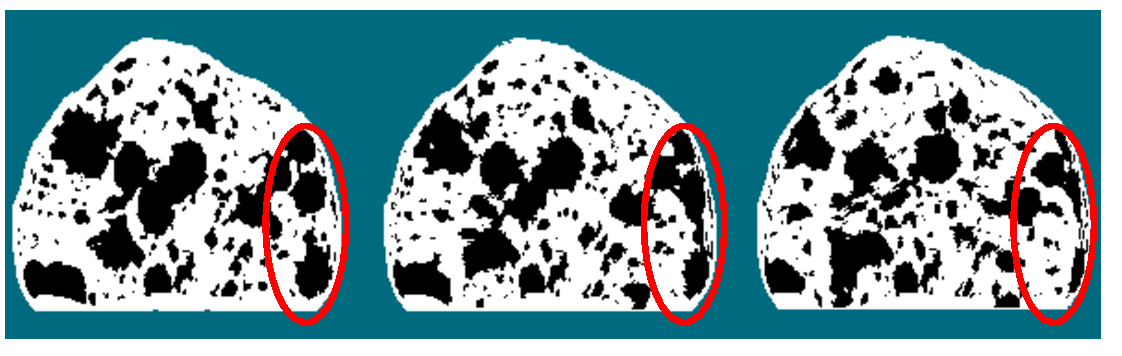
\includegraphics[width=13cm]{figures/parameterp}
\caption{Efecto del parámetro $p$: de izquierda a derecha $p$ es $0$, $5$, $10$,$15$, y $25$, respectivamente.}
\label{fg:parameterp}
\end{figure*}


\subsection{Formación de la Corteza}
El modelo de cocción que hemos introducido no incluye detalles precisos de la formación de la corteza.
En estas ecuaciones, la corteza se asume es producida en la superficie del material, a determinada temperatura, pero esta simplificación está lejana a lo que ocurre actualmente en el proceso real de cocción.
La literatura de ingeniería de los alimentos define la corteza como una interfase que emerge entre la masa y el aire.
Entre sus principales características se encuentra la formación de un material más denso en la superficie, y una diferenciación de color.
Sin embargo, los detalles precisos acerca de cómo esto ocurre se desconocen, por lo tanto, la apariencia exacta de la misma, está lejos de ser comprendida en los modelos presentes acutalmente.

Debido a esto, y basados en la aproximación inicial asumida, utilizamos el campo escalar de distancias computado previamente para definir una región de corteza.
Esta elección está fundada en el hecho de que la corteza está mayormente determinada por un frente de evaporación que resulta de la temperatura \cite{Jefferson2007}.
En otras palabras, obtenemos las posiciones utilizando el campo escalar mencionado, ya que hemos definido una relación entre la temperatura y la distancia a la superficie.
Además, obtenemos diferentes apariencias de pan utilizando un parámetro de distancia que determina diferentes anchos de corteza.

También, por completitud, presentamos otro método para calcular la misma.

\paragraph{Determinación de la corteza utilizando morfología matemática}
Debido a que es difícil o imposible definir funciones matemáticas algebraicas que se adapten a cualquier forma, proponemos un método automático para determinar regiones del volumen utilizando el formalismo conocido como morfología matemática \cite{Gonzalez2001}.

Con esto, se presente obtener una región que se ajuste a los bordes del campo escalar.
Para esto se utilizarán técnicas simples conocidas como apertura, cierre, erosión y dilatación.

Las operaciones las definiremos en campos escalares tridimensionales.
Un elemento estructurante $E$ es un campo escalar binario que representa una forma particular (cubo, esfera, etc.).
Los elementos estructurantes son utilizados en la definición de las operaciones antes mencionadas.
La operación de erosión se utiliza para reducir el tamaño total del campo escalar.
La erosión de un campo escalar $A$ utilizando un elemento estructurante $B$ es definida de la siguiente manera,

\begin{equation}
A \ominus B = \{z\in \mathbb{Z}^3 | B_{z} \subseteq A\},
\end{equation}

\noindent donde $B_{z}$ es la traslación de $B$ por el vector tridimensional$z$.

La dilatación es una operación utilizada para aumentar el tamaño total del campo escalar, siguiendo sus bordes.
La dilatción de un campo escalar $A$ utilizando el elemento estructurante $E$ es definida como sigue,

\begin{equation}
A  \oplus E = \bigcup_{e\in E} A_e.
\end{equation}

La operación de cierre es utilizada para cerrar {\em agujeros} en el campo escalar.
El cierre de un campo $B$ utilizando un elemento estructurante $E$ es definido como una dilatación seguida de una erosión,

\begin{equation}
B \bullet E = (B \oplus E) \ominus E,
\end{equation}

ver \cite{Gonzalez2001} para obtener mayores detalles.

Para obtener la región externa de la geometría representada en el campo escalar, hay que eliminar los agujeros internos que representan las burbujas y luego computar el borde.
Para esto, el primer paso produce un cierre $c$ del campo escalar utilizando un cubo (elemento estructurante de radio $r$), causando el cierre de las burbujas internas.
Llamaremos $d$ a la dilatación de $c$ con un elemento esférico de radio $r_{2}$ y $e$ a la erosión $d$ utilizando un elemento estructurante esférico con un radio ligeramente menor($r_{3}$).
La diferencia entre $d$ y $e$ ($d-e$) se encuentra en el borde del campo escalar, por lo cual puede utilizarse como corteza.
Para eliminar posibles imperfecciones en los pasos anteriores, se suaviza el campo escalar por medio de un cierre de $d-e$ y una dilatación del resultado, obteniendo la corteza final.


La Fig.~\ref{fg:crusts} muestra ejemplos de campos escalares con cortezas agregadas utilizando este técnica. Los resultados se adaptan naturalmente a cualquier campo escalar, inclusive si existen agujeros grandes.
El resultado cubre completamente el campo escalar, por lo cual para poder observar la parte interna del material deben realizarse cortes en el mismo.

\begin{figure}
  \centerline{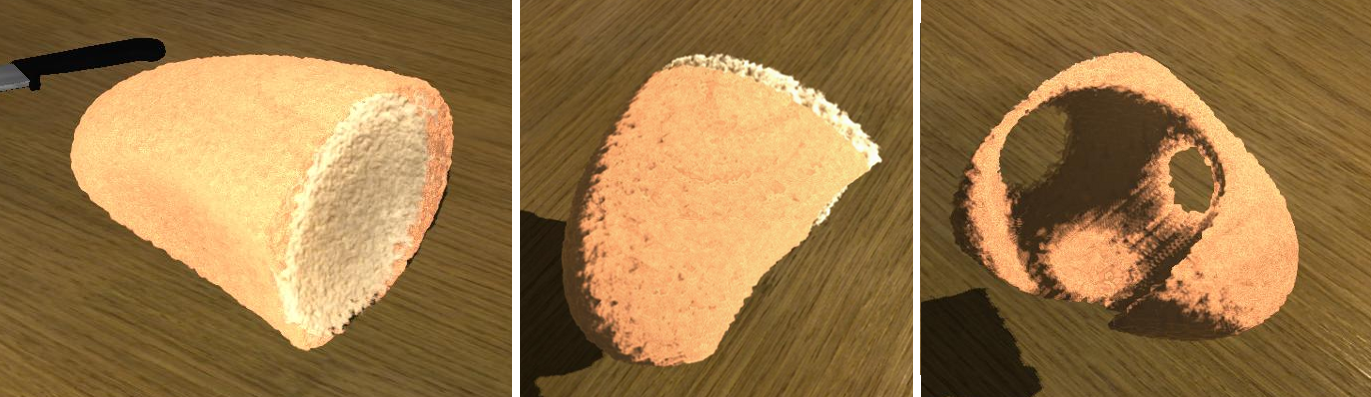
\includegraphics[width=13cm]{figures/crusts}}
  \caption{Determinación de la corteza del pan utilizando morfología matemática. La imagen de la derecha muestra que el método de utilización de morfología matemática funciona incluso cuando existen grandes agujeros en el campo escalar.}
  \label{fg:crusts}
\end{figure}

\subsection{Tiempos de cómputo}
En la implementación utilizamos Python\footnote{python.org} y Cython\footnote{cython.org}.
En la Tabla~\ref{tab:computingtimes} se muestran tiempos de cómputo típicos para los distintos pasos en la simulación de la formación del pan, detallados en secciones anteriores. %In addition, rendering times with DVR are in the order of $~300$ ms (milliseconds), achieving interactive framerates.

\begin{table}[h!]
       % Give a unique label
% For LaTeX tables use
\begin{tabular}{lllll}
\hline\noalign{\smallskip}
Resolución del Campo Escalar & $256^{3}$ & $384^{3}$  & $512^{3}$ \\
\noalign{\smallskip}\hline\noalign{\smallskip}
Leudado & 0.28 & 0.97 & 2.29 \\
Intersección & 8 & 10.81 & 14.97 \\
Campo escalar de Distancias & 7 & 23.73 & 56 \\
Cocción & 19.92 & 51.15 & 117.27 \\
%Rendering & 1s & 4s & 0\% \\
\noalign{\smallskip}\hline
\end{tabular}
\caption{Tiempos de cómputo típicos en nuestro modelo expresados en segundos.}
\label{tab:computingtimes}
\end{table}

Es importante mencionar que la mayor parte del tiempo de cómputo en la cocción está dedicado al cómputo del gradiente, y no al proceso de cocción en sí.
Debido a los costos computacionales en resoluciones superiores, el usuario puede generar vistas previas de los panes utilizando campos escalares con menores resoluciones.


\section{Resultados}
En esta sección presentamos imágenes renderizadas de geometrías de pan obtenidas utilizando nuestro modelo.

Las Figs.~\ref{fg:renders}, \ref{fg:renders2}, y ~\ref{fg:renders3} muestran imágenes renderizadas de panes obtenidos en este trabajo.
Las Figs.~\ref{fg:renders} y ~\ref{fg:renders2} marcan las diferencias en realismo entre resoluciones del campo escalar de ($256^{3}$) y  ($512^{3}$) respectivamente.
La Fig.~\ref{fg:renders3} muestra versiones de alta resolución en el campo escalar de otras geometrías, incluyendo panes con formas de conejos.
La Fig.~\ref{fg:croissant} muestra un pan con forma de {\em croissant} en el cual se han hechos distintos cortes, los cuales demuestran que el método permite obtener imágenes de partes arbitrarias del material.
Las Figs.~\ref{fg:bigalveoli} y ~\ref{fg:bakedbunny} muestran un pan típico y uno con forma de conejo, mostrando burbujas grandes y las burbujas deformadas como resultado del proceso de cocción.
Además se cambió el color de la miga.

Los colores de corteza y miga son parámetros definibles por el usuario. Los cortes en la miga son fácilmente producidos cambiando a $0$ las regiones deseadas en el campo escalar luego de la cocción, y antes del renderizado.

\begin{figure*}[!ht]
\begin{center}
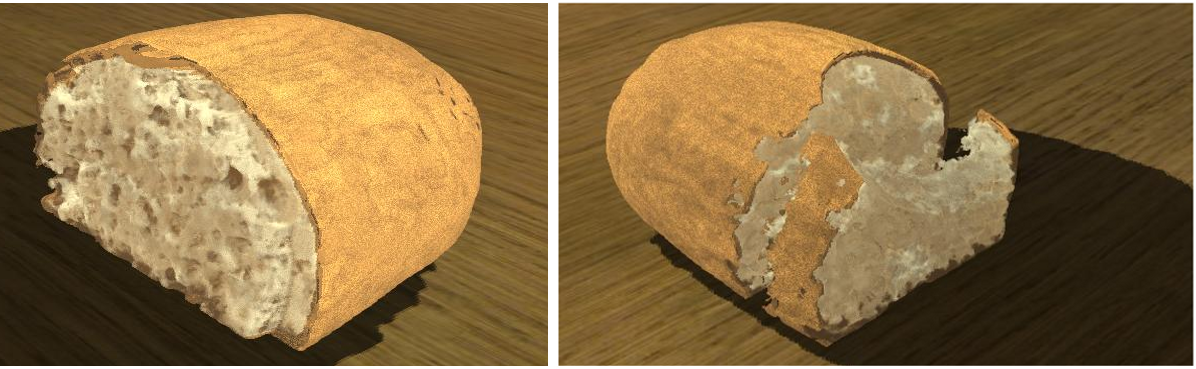
\includegraphics[width=13cm]{figures/otherbread}
\caption{Cortes de pan luego de la cocción, utilizando un campo escalar de dimensiones $256^{3}$. Las imágenes muestran que la miga y la corteza son consideradas en nuestro modelo.}
\label{fg:renders}
\end{center}
\end{figure*}

\begin{figure*}[!ht]
\begin{center}
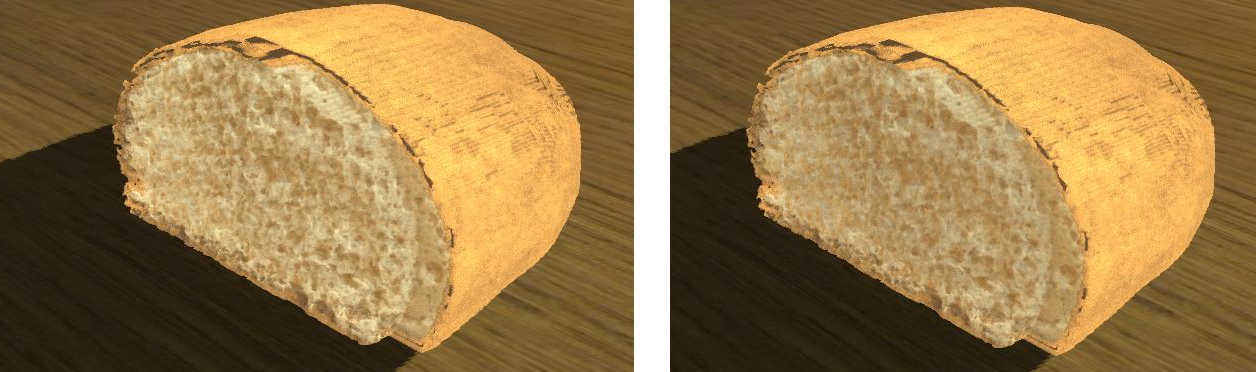
\includegraphics[width=13cm]{figures/otherbread512}
\caption{Cortes de pan luego de la cocción, utilizando un campo escalar de dimensiones $512^{3}$. Se observan mayores detalles en la miga, lo cual aumenta el realismo de la imagen.}
\label{fg:renders2}
\end{center}
\end{figure*}

\begin{figure*}[!ht]
\begin{center}
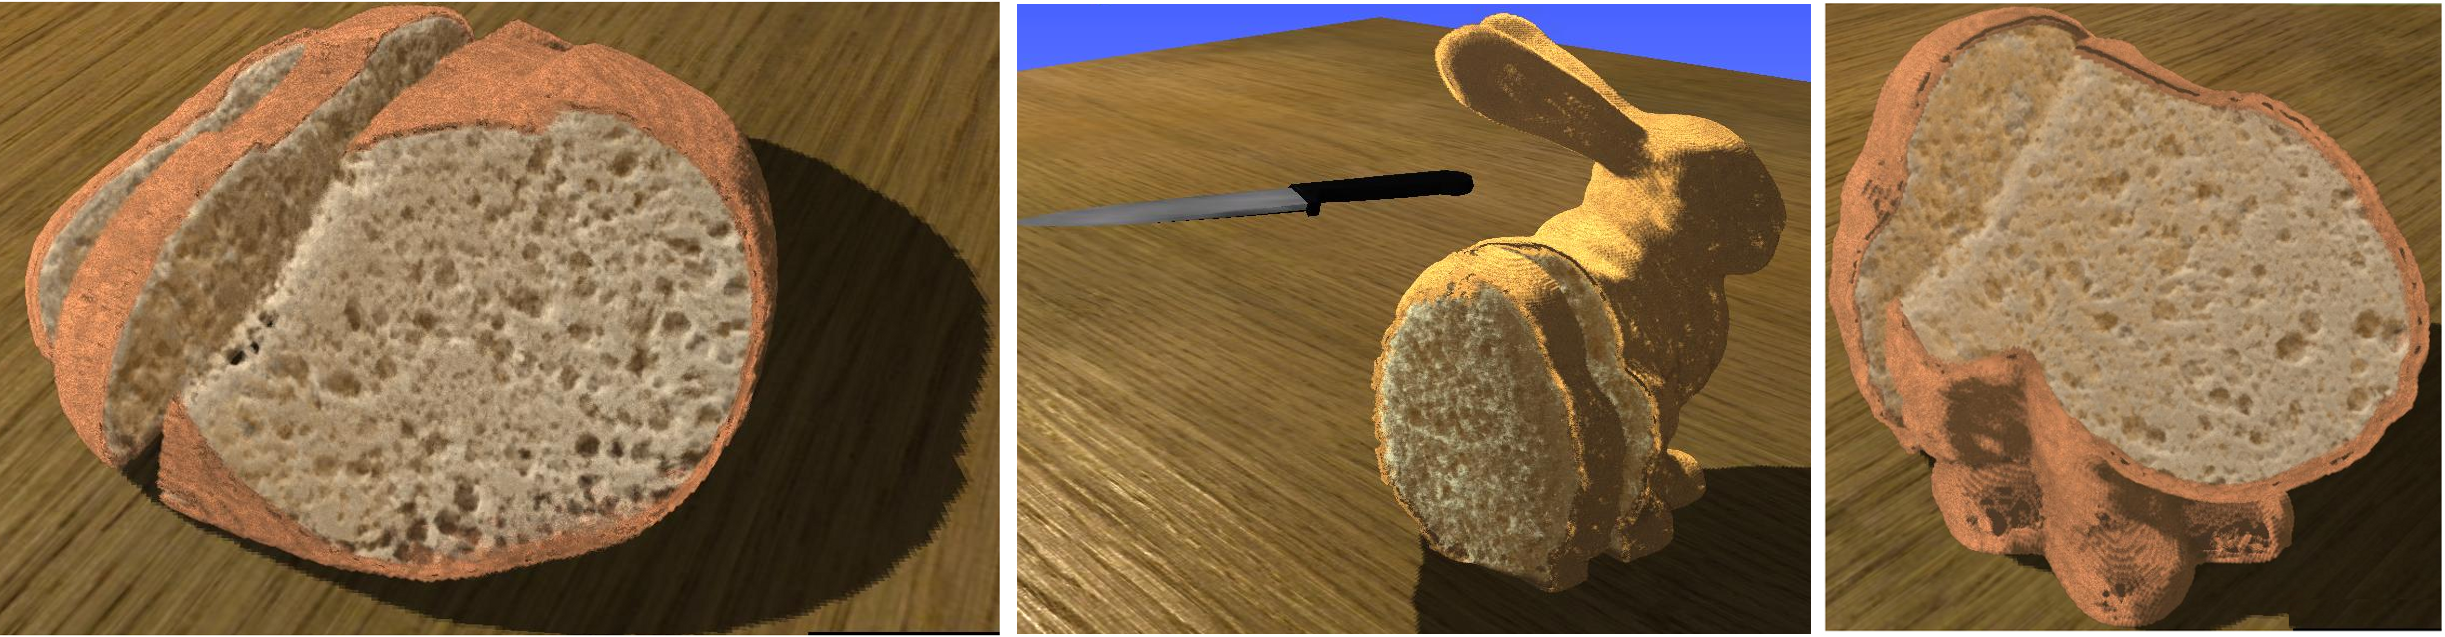
\includegraphics[width=13cm]{figures/final}
\caption{Cortes de pan luego de la cocción con distintas geometrías.}
\label{fg:renders3}
\end{center}
\end{figure*}

\begin{figure*}[!ht]
\begin{center}
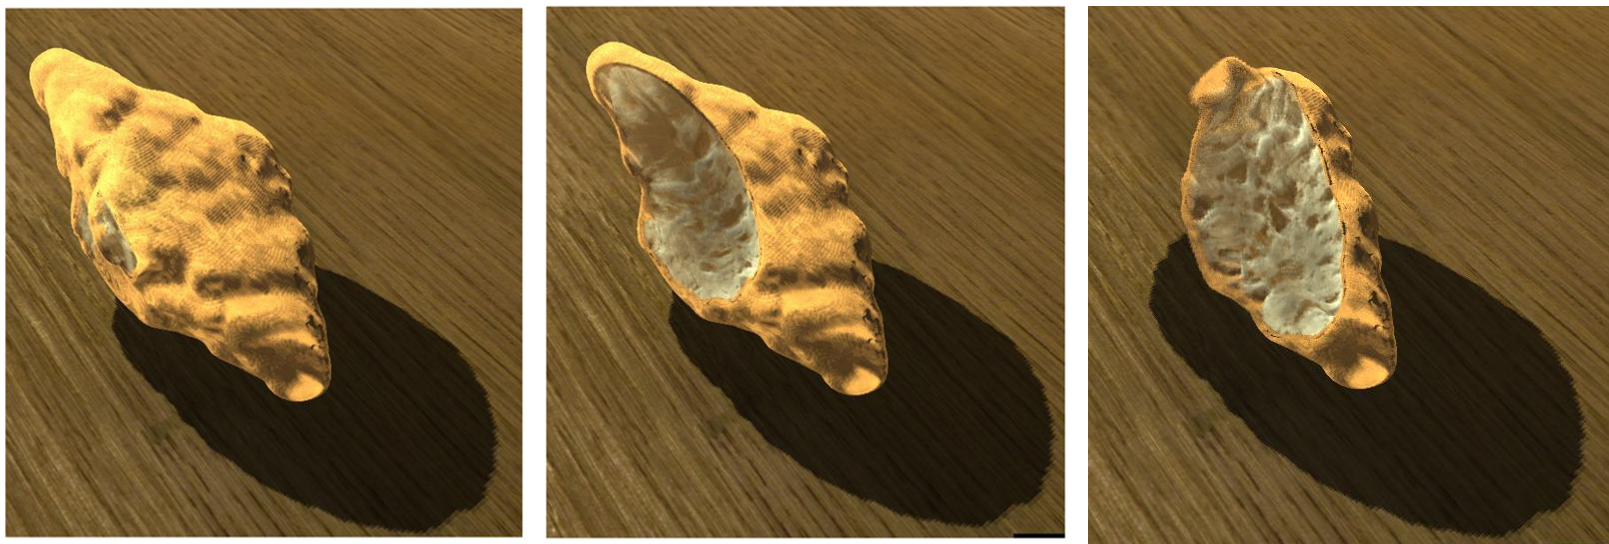
\includegraphics[width=13cm]{figures/croissant}
\caption{Cortes de una Croissant luego de la cocción. La imagen muestra el interior de la miga en distintas regiones del volumen.}
\label{fg:croissant}
\end{center}
\end{figure*}

\begin{figure*}[!ht]
\begin{center}
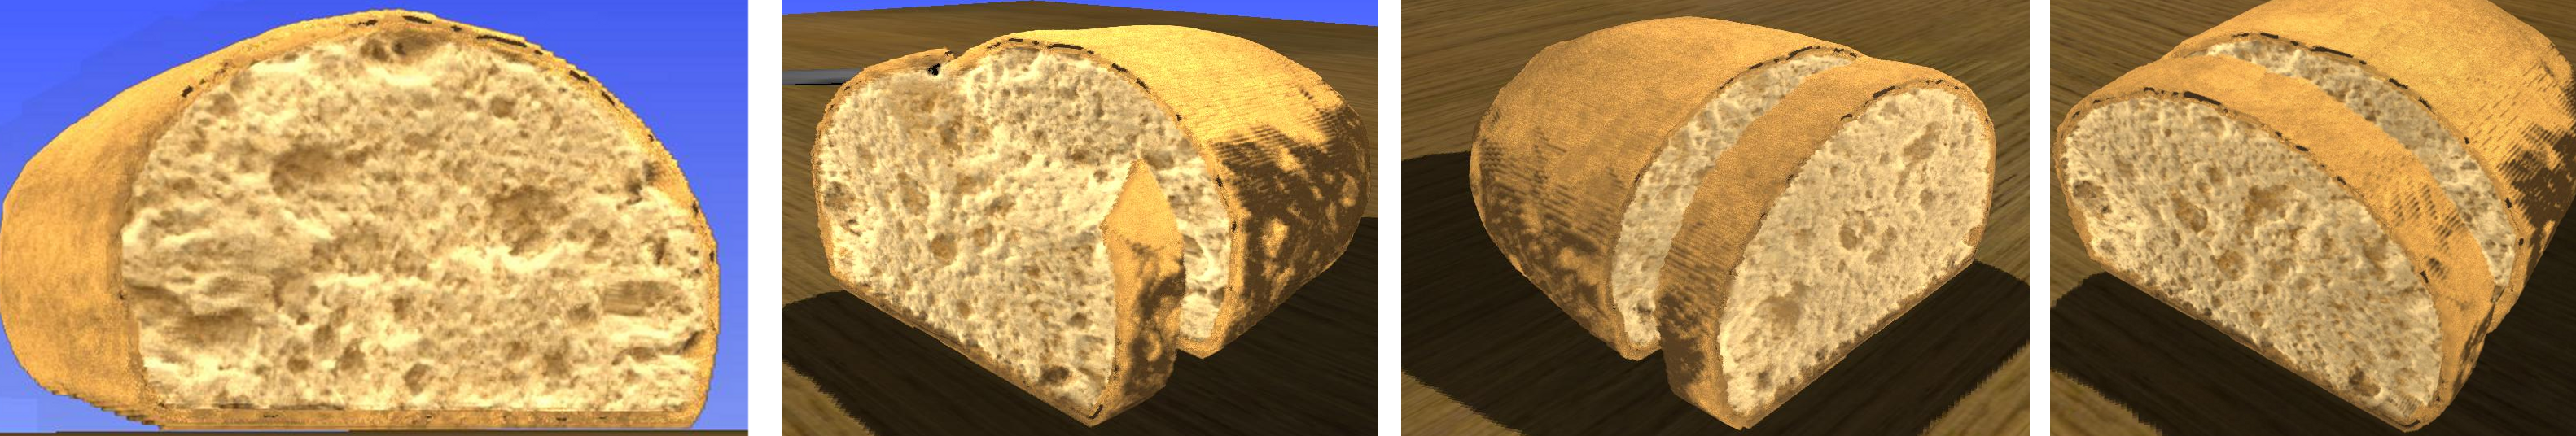
\includegraphics[width=13cm]{figures/baked}
\caption{Cortes de pan luego de la cocción, con burbujas de mayor tamaño, como es típico en determinados panes reales.}
\label{fg:bigalveoli}
\end{center}
\end{figure*}

\begin{figure*}[!ht]
\begin{center}
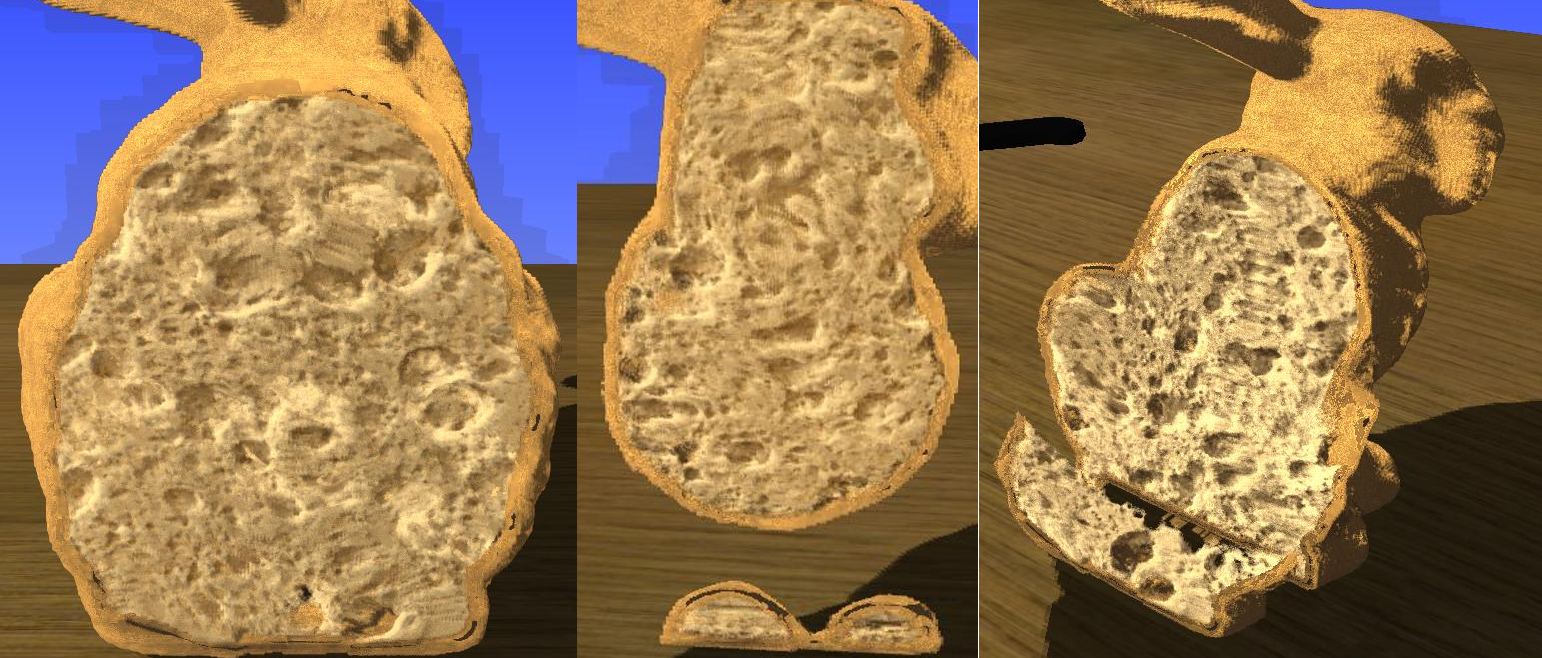
\includegraphics[width=13cm]{figures/bakedbunny}
\caption{Cortes de pan luego de la cocción con burbujas de mayor tamaño. Además, puede observarse más claramente el efecto de la cocción en la deformación de las burbujas, las cuales tienden a seguir la forma de la corteza.}
\label{fg:bakedbunny}
\end{center}
\end{figure*}

%Images show realistic bread appearances, suitable for photo-realistic rendering and serious ga\-mes \cite{Susi2007}. 


%This is illustrated in Figure~, where arrow lengths indicate vector modulus. The image shows that the field's influence is higher near the crust, mostly deforming outer bubbles. This behavior is consistent with real bread crumbs: baking influences the outer bubbles' shape, elongating them parallel to the crust \cite{Scanlon2001}, in other words, following its isotherms.


%\subsection{Leudado}
%El leudado es el principal responsable de la apariencia visual de las burbujas en la miga de pan \cite{}.

%Los patrones observados en la distribución de las burbujas son resultado de procesos complejos, entre los que encontramos reacciones químicas y deformaciones físicas. Este paso en la fabricación consiste en un crecimiento libre de las burbujas, producido por organismos vivos (levadura) en la masa sin cocción del pan.

%Diferentes estudios fenomenológicos de la distribución de burbujas aparecen en la literatura. Los mismos utilizan tomografía de rayos X y extracción de características sobre imágenes para obtener una imagen y modelar las mismas \cite{Babin2006,Gonzales2008,VanDyck2014}.

%El modelo utilizado está inspirado en un modelo propuesto en \cite{Mandelbrot1983}, el cual intenta modelar quesos y distribuciones de cráteres en cuerpos celestes. Validaremos la distribución obtenida utilizando una métrica multi-fractal basada en el espectro multifractal Sandbox.

%Se comienza con una esfera de radio $v = 1$ voxels. Este radio es incrementado en cada iteración. En cada paso, se extraen un número de esferas proporcional al radio:


%\begin{equation}
%N_{esferas} = \frac{k}{r^{d}},
%\end{equation}

%\noindent donde $k$ y $d$ son parámetros con valores reales, y $r$ es el radio de la esfera.

%La Figura~\ref{FigProving} muestra un ejemplo en dos dimensiones de este proceso, donde $d$ controla la relación existente entre los radios de las esferas y $k$ el número de esferas que extraemos en cada paso.

%Las imágenes muestran una apariencia similar a las que pueden observarse en diferentes espumas (café, jabón, cerveza), y en particular a la que muestra el leudado del pan \cite{Babin2006}. 

%\begin{figure}
%\includegraphics[scale=0.28]{bubbles.png}
%\caption{Fractal bread proving simulation.}
%\label{FigProving}
%\end{figure}

%En la sección de validación ajustaremos los parámetros para adecuarlos a los de imágenes de migas reales de pan.

%\subsection{Cocción}
%\subsubsection{Modelo Matemático}

%El modelo matemático del proceso de cocción simula la transferencia de calor y masa en diversos alimentos, entre ellos el pan.  En esta tesis utilizaremos modelos de una dimensión~\cite{Thorvaldsson1999,Purlis2010}. Por ejemplo, Purlis~\cite{Purlis2010} modela la geometría del pan como un cilindro infinito.

%Utilizaremos la solución numérica presente en {Thorvaldsson and Janestead \cite{Thorvaldsson1999} and Powathil~\cite{Powathil2004}. La misma modela el problema como un conjunto de tres ecuaciones diferenciales acopladas que describen transferencia de calor, difusión de vapor de agua y difusión de agua. Sólo será tenida en cuenta la temperatura ($T$) como entrada en el pipeline de generación de pan.
%The paper defines the geometry as a prism of dimensions $12\times12\times2~cm^{3}$, with  $x$ (the shortest side) as the coordinate of interest.


%La siguiente ecuación modela la transferencia de calor en la masa de pan a través de un balance de energía y de evaporación de agua debido a la temperatura~\cite{Thorvaldsson1999}:
%
%\begin{equation}
%\frac{\partial T}{\partial t} = \frac{1}{\rho C_{p}} \frac{\partial}{\partial x} \left ( k \frac{\partial T}{\partial x} \right ) + \frac{\lambda}{C_{p}} \frac{\partial W}{\partial t}+\frac{\lambda W}{ C_{p} \rho}\frac{\partial \rho}{\partial t}
%\end{equation}
%
%donde $T$ es la temperatura, $x$ ies la coordenada radial, $C_{p}$ es calor específico, $\rho$ es la densidad, $k$ es la conductividad térmica, $\lambda$ es el calor latente de evaporación de agua, y  $W(x;t)$ es el contenido de agua líquida. Las condiciones iniciales:
%
%\begin{align}
%T(x,0) &= T_{0}(x), 0\le x \le L/2
%\end{align}
%y las condiciones de borde completan el modelo:
%\begin{align}
%\left ( \frac{\partial T}{\partial x} \right )_{x=L/2} &= 0 , t > 0 \\
%-k \left ( \frac{\partial T}{\partial x} \right )_{x=0} &= h_{r}(T_{r}-T_{s}) + h_{c}(T_{air}-T_{s}) - \lambda \rho D_{w} \left (\frac{\partial W}{\partial x} \right )_{x=0}
%\end{align}
%
%donde $h_{r}$ y $h_{c}$ son subtérminos del coeficiente de transferencia de calor ($h = h_{r}+h_{c}$), $T_{air}$, $T_{s}$, $T_{r}$ son las temperaturas en el aire, en la superficie del pan y en la fuente de radiación, respectivamente, $L$ es la altura del pan ($x = L/2$ es el centro del pan y $x = 0$ es el borde del pan), y $T_{0}$ es la temperatura inicial. Las temperaturas se expresan en Kelvin ($K$).  Además el modelo presenta ecuaciones similares para la difusión de vapor de agua ($W$) y la difusión de agua líquida ($V$). Más detalles del modelo pueden ser encontrados en \cite{Thorvaldsson1999}.

%Utilizamos este modelo para obtener un mapa de temperaturas sobre el volumen del pan al final del proceso de cocción. Estas temperaturas se utilizarán para deformar la geometría de las burbujas resultantes del proceso de leudado.



%El modelo matemático del proceso de cocción es un modelo $3D$ que, en su versión más simple involucra transferencia de calor y de masa.

%El proceso de creación de pan real sitúa a la cocción luego de la deformación de la masa. Esto supone geometría arbitraria en los bordes de la masa. El proceso de cocción debe amoldarse a estas condiciones arbitrarias, lo cual hace que el modelo resulte complejo. Para simplificar esto, proponemos aplicar la cocción antes de deformar la masa original. Esta simplificación resulta adecuada para nuestros propósitos y es validada posteriormente.


%Además, para nuestros propósitos la inclusión de un modelo completo $3D$ resulta excesiva dado su costo computacional y el limitado impacto final sobre la estructura que pretendemos modelar. Por estas razones elegimos un modelo cilíndrico unidimensional, el cual se extiende fácilmente a $3$ dimensiones. A pesar de esta simplificación, la literatura muestra que el modelo captura los detalles esenciales en la transferencia de calor y masa \cite{Purlis2010,Powathil2004}.

%La implementación numérica del modelo está descrita en \cite{Powathil2004}. La misma usa el esquema de diferencias finitas. El horno en el cual se sitúa el pan se establece a $210  ^{\circ}C$ y el tiempo es discretizado en intervalos de tiempo de duración $\Delta t = 0.05s$. El algoritmo devuelve un arreglo $Temp$ de $N_{grid}$ valores de temperatura. Cada valor representa una posición en la masa luego de $M$ pasos temporales. Por cuestiones de estabilidad definimos el tamaño de la grilla como $N_{grid}=32$ e interpolamos los valores de temperatura para obtener mayores resoluciones ($N_{im}$).

%El vector obtenido presenta temperaturas decrecientes de $R = 0$ a $R = L/2$, debido a que el centro del pan presenta las menores temperaturas ($R=L/2$), a diferencia de los bordes ($R=0$) los cuales poseen una distancia menor a la fuente de calor. De esta manera, $Temp[L/2]$ corresponde a $x = N_{im}/2, y=N_{im}/2$ y $Temp[0]$ corresponde a los $(x,y)$ lejos del centro del cilindro. 

%Luego de interpolar las temperaturas traducimos el vector $Temp_{int}$ a coordenadas $2D$ mediante las siguientes relaciones:
%\begin{align}
%\displaystyle I(\frac{N_{im}}{2}-i,\frac{N_{im}}{2}-j) &= Temp_{int}[L/2-R], \\
%R &= \sqrt{i^{2}+ j^{2}}, \\
%i, j &\in [-\frac{N_{im}}{2},\frac{N_{im}}{2}],
%\end{align}


%\noindent donde $R$ es el índice del vector, y $x$ e $y$ son coordenadas $2D$ en la imagen de destino, en otras palabras, el píxel $I(N_{im}/2-i,N_{im}/2-j)$ es seteado con el valor $Temp_{int}[L/2-R]$. Finalmente obtenemos una imagen cuadrada de lado $N_{im}$. La figura ~\ref{FigBakingVectorField} muestra un ejemplo de dicha imagen.

%A partir de esta imagen obtenemos su gradiente \cite{Gonzalez2006} para  computar un campo vectorial $[g_{x},g_{y}]$, utilizándolo para deformar posteriormente la textura volumétrica de la siguiente manera:

%\begin{align}
%\displaystyle u = x+p*dist_{xy}*g_{x}[x,y],\\
%v = y+p*dist_{xy}*g_{y}[x,y],
%\end{align}
%\noindent donde $(u,v)$ son las coordenadas en el volumen deformado, ($x,y$) son las coordenadas originales, $p$ es parámetro real positivo que sirve para modular el efecto del campo en el volumen, y $dist_{xy}$ es la distancia euclídea de $(x,y)$ al centro del cilindro ($\sqrt((x-N_{x}/2)^{2}+(y-N_{y}/2)^{2})$). 


%El parámetro distancia al centro es útil para remarcar las diferencias existentes en el efecto que produce el proceso de cocción sobre las burbujas en distintas zonas de la masa.
%La Figura~\ref{FigBakingVectorField} muestra además el vector gradiente superimpuesto sobre la imagen. En nuestros experimentos encontramos que $p=10$ es suficiente para producir un efecto apreciable sobre las burbujas.
%El procedimiento de cocción reduce aproximadamente a la mitad el tamaño total de la imagen.



%\begin{figure}
%\centering
%\includegraphics[scale=0.58]{vfield.png}
%\caption{Temperaturas obtenidas sin interpolar a partir del modelo matemático de cocción del pan y vector gradiente superimpuesto}
%\label{FigBakingVectorField}
%\end{figure}

%El largo de las flechas indica el módulo del vector. La imagen muestra que la influencia del campo es mayor cerca de la corteza del pan, lo cual se condice con el efecto observable en panes reales. El proceso de cocción elonga paralelamente a la corteza las burbujas del material \cite{Scanlon2001} (siguiendo las isotermas).

%Siguiendo el modelo cilíndrico, cada rodaja (representada por un volumen de altura $1$ vóxel) es deformado independientemente utilizando el mismo procedimiento. La Figura~\ref{FigBaking} muestra un ejemplo de rodaja luego de la cocción digital.

%Cabe mencionar que se intentó interpolar la imagen resultante en lugar del vector original de temperaturas, pero el campo vectorial resultante tenía vectores de módulos cercanos a cero.

%\begin{figure}
%\begin{center}
%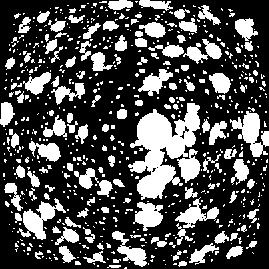
\includegraphics[scale=0.8]{baking.png}
%\caption{Corte del volumen luego de la cocción. Las burbujas siguen un campo vectorial concéntrico.}
%\label{FigBaking}
%\end{center}
%\end{figure}


%\subsection{Intervención Humana en el Proceso}

%\subsubsection{Mean Value Coordinates}

%Para permitir una interacción con el modelado del pan sintético, se definen puntos de control que el usuario puede mover a voluntad para deformar localmente la masa. Para esto se utiliza Mean Value Coordinates (MVC), el cual es un método poderoso en animación \cite{Floater2003,Floater2005,Ju2005}.
%Este método computa coordenadas baricéntricas a partir de los puntos de control sin deformar (una caja que rodea al objeto) con las cuales calcula las posiciones destino de los puntos de interés en el dominio (en nuestro caso, cada pixel de la imagen es un punto de interés).

%El método usa dos conjuntos de puntos de control para realizar la deformación. El primero ($cageOrig$) es un conjunto de puntos que se sitúa en el borde de la imagen original. Cada texel computa su coordenada baricéntrica con respecto a estos puntos. Cuando movemos estos puntos formamos el vector $cageNew$. Para cada píxel $(x,y)$ el método computa las coordenadas baricéntricas del mismo con respecto a la caja original, multiplicando las mismas con los puntos de control deformados. El resultado $(u,v)$ se utiliza como coordenadas en la imagen original para setear el valor que debe tomar el píxel actual:
%\begin{align}
%barycoords &= bary([x,y],cageOrig),\\
%(u,v) &= \sum_{i} {barycoords_{i} * cageNew_{i}}, \\
%T_{new}(x,y) &= T_{orig}(u,v).
%\end{align}
%As the reader will see in next sections, this method produces realistic-looking deformations.

%====================================================================

%Durante el proceso de fabricación del pan, la masa sufre transformaciones que incluyen la intervención del ser humano, el cual busca distribuir la levadura de manera homogénea por medio de deformaciones.

%En nuestro modelo, permitimos que un artista pueda definir puntos de control en una imagen para modificar la silueta externa de la masa. Siguiendo el modelo cilíndrico, la deformación en esta etapa se aplica a cada corte $2D$ del volumen.

%La Figura~\ref{FigMVC} muestra un ejemplo de deformación utilizando Mean Value Coordinates. En este caso se necesitaron solamente $11$ puntos de control (rojo) para aproximar la silueta de la corteza. La FIgura~\ref{FigMVCpoints} muestra los puntos de control y la caja deformada En el ejemplo definimos un mayor número de puntos de control en la región de interés (derecha) para producir una silueta más controlada.

%\begin{figure}[!ht]
%\includegraphics[scale=0.65]{warping.png}
%\caption{Comparación entre pan real (izquierda) y sintético utilizando la deformación por MVC (derecha).}
%\label{FigMVC}
%\end{figure}


%\begin{figure}[!ht]
%\includegraphics[scale=1.35]{warppoints.png}
%\caption{Imagen deformada utilizando MVC: puntos de control sin modificar (verde) puntos de control modificados (rojo). Otras líneas indican desplazamiento de puntos. }
%\label{FigMVCpoints}
%\end{figure}


%This method also warps the bubbles' shape. The deformed bubbles have a natural appearance in concordance with real bread bubbles. 
\section{Conclusiones}
En este Cap\'itulo hemos introducido diversos algoritmos para subsanar la falta de procedimientos flexibles e intuitivos para modelar determinados materiales, entre ellos materiales porosos como el pan. Además, como subproducto de la investigación, se obtuvieron representaciones bidimensionales de madera, granito, mármol y otros materiales comunes en la literatura.
Hemos demostrado visualmente la capacidad de los métodos.

El primer aporte es un algoritmo que produce texturas bidimensionales de materiales conocidos como madera y granito, utilizando sistemas de partículas, el cual fue presentado en una conferencia local \cite{Baravalle2011}.

Haciendo hincapié en materiales porosos, particularmente el pan, diseñamos algoritmos que utilizan sistemas de partículas en conjunción con Sistemas Dinámicos para producir texturas que representan de manera realista geometrías de pan, el cual fue presentado en un congreso y revista nacionales \cite{Baravalle2014}.

Finalmente, utilizando como referencia el proceso de formación real del pan, utilizamos conocimientos de ingeniería de los alimentos para producir una secuencia de pasos que emulan el proceso real de formación del pan.
El mismo permite modelar de manera realista tipos de panes arbitrarios, produciendo geometrías de su miga y su corteza, utilizando un proceso fractal de generación.
Para ello, emulamos un proceso de leudado configurable por el usuario, tanto en forma global, supliendo una geometría arbitraria en tres dimensiones, como en el burbujeado interno, por medio de parámetros intuitivos de generación (radio máximo y mínimo de las burbujas, cantidad de burbujas, etc.).
Luego aplicamos una simulación física de la cocción que deformó ligeramente las burbujas.
Finalmente, la corteza fue generada sobre la superficie del material.
El algoritmo de renderizado utilizado será explicado en el siguiente capítulo, el mismo produjo imágenes realistas de diversos tipos de pan, en varias etapas del proceso de formación del mismo.

El modelo introducido es más flexible y poderoso que el estado del arte actual en modelado de geometría de materiales porosos y panes.

En un capítulo posterior, y con intención de validar el procedimiento, mostraremos que las geometrías obtenidas por el método inspirado en el proceso de formación del pan, arrojan distribuciones de burbujas coincidentes con panes reales.

